\documentclass[11pt]{article}
\usepackage{amsfonts}
\usepackage{amsmath}
\usepackage{amsthm}
\usepackage{amssymb}
\usepackage{mathrsfs}
\usepackage[fit]{truncate}
\usepackage{acl2012}
\usepackage{times}
\usepackage{latexsym}
\usepackage{amsmath}
\usepackage{url}
\usepackage{graphicx}
\usepackage{caption}
\usepackage{multirow}
\usepackage{colortbl}
\usepackage{dblfloatfix}
\usepackage{float}
\usepackage{subfloat}
\usepackage{booktabs}
\usepackage{subcaption}

\DeclareMathOperator*{\argmax}{arg\,max}
\setlength\titlebox{5cm}    % Expanding the titlebox

\newcommand{\affliationPenn}{\ensuremath{{}^\text{1}}}
\newcommand{\affliationJHU}{\ensuremath{{}^\text{2}}}

\title{A large scale study of the languages spoken (by bilinguals) on Mechanical Turk}
\title{The Language Demographics of  Amazon Mechanical Turk}

\author{Ellie Pavlick\affliationPenn \ \ \ \ \ Matt Post\affliationJHU \ \ \ \ \  Ann Irvine\affliationJHU  \ \ \ \ \ Dmitry Kachaev\affliationJHU  \ \ \ \ \  Chris Callison-Burch\affliationPenn$^{,}$\affliationJHU \\
\affliationPenn Computer and Information Science Department, University of Pennsylvania \\
\affliationJHU Human Language Technology Center of Excellence, Johns Hopkins University \\
  }
  

\date{}

\begin{document}
\maketitle

\begin{abstract}
We present a large scale study of the languages spoken by bilingual workers on Mechanical Turk (MTurk).  
We establish a  methodology for determining the language skills of anonymous crowd workers that is more robust than simple surveying.  We validate workers' self-reported language skill claims by measuring their ability to correctly translate words, and by geolocating workers to see if they reside in countries where the languages are likely to be spoken. Rather than posting a one-off survey, we posted paid tasks consisting of 1,000 assignments to translate a total of 10,000 words in each of 100 languages.  Our study ran for several months, and was highly visible on the MTurk crowdsourcing platform, increasing the chances that bilingual workers would complete it.  Our study was useful both to create bilingual dictionaries and to act as census of the bilingual speakers on MTurk.  We use this data to recommend languages with the largest speaker populations as good candidates for other researchers who want to  develop crowdsourced, multilingual technologies. To further demonstrate the value of creating data via crowdsourcing, we hire workers to create bilingual parallel corpora in six Indian languages, and use them to train statistical machine translation systems. 

\end{abstract}

\section{Overview}
Crowdsourcing is a promising new mechanism for collecting data for natural language processing research. Access to a fast, cheap, and flexible workforce allows us to collect new types of data, potentially enabling new language technologies.
Because crowdsourcing platforms like Amazon Mechanical Turk (MTurk) give researchers access to a worldwide workforce, one obvious application of crowdsourcing is the creation of multilingual technologies. 
With an increasing number of active crowd workers located outside of the United States, there is even the potential to reach fluent speakers of lower resource languages.
In this paper, we investigate the feasibility of hiring language informants on MTurk by conducting the first large-scale demographic study of the languages spoken by workers on the platform. 

There are several complicating factors when trying to take a census of workers on MTurk.  The workers' identities are anonymized, and Amazon provides no information about their countries of origin or their language abilities.  Posting a simple survey to have workers report this information may be inadequate, since (a) many workers may never see the survey, (b) many opt not to do one-off surveys since potential payment is low, and (c) validating the answers of respondents is not straightforward. 

Our study establishes a methodology for determining the language demographics of anonymous crowd workers that is more robust than simple surveying. We ask workers what languages they speak and what country they live in, and validate their claims by measuring their ability to correctly translate words and by recording their geolocation.  To increase the visibility and the desirability of our tasks, we post 1,000 assignments in each of 100 languages.  These tasks each consist of translating 10 foreign words into English.  Two of the 10 words have known translations, allowing us to validate that the workers' translations are accurate.  We construct bilingual dictionaries with up to 10,000 entries, with the majority of entries being new. 


%%%%%%%%%%%%%%% MAP OF WORKER LOCATIONS %%%%%%%%%%%
\begin{figure*}[h]
\centering
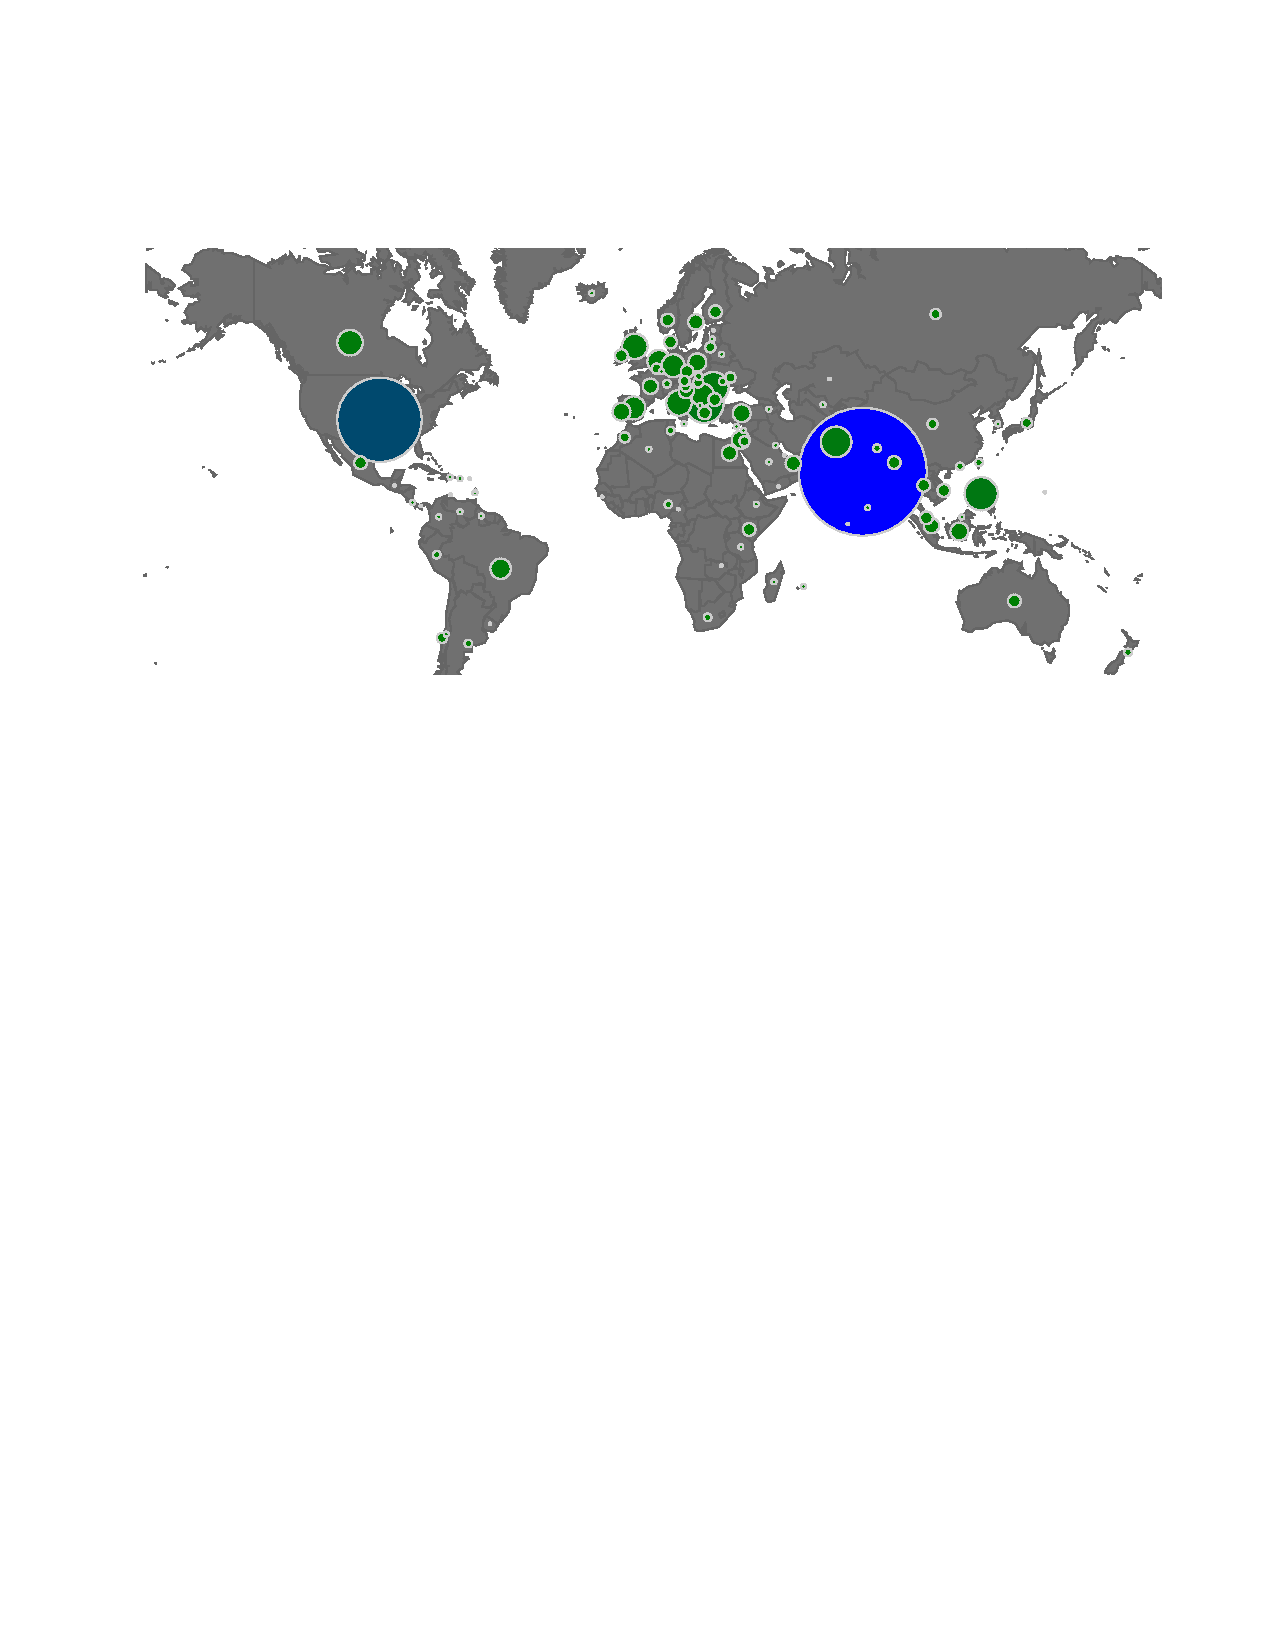
\includegraphics[width=\linewidth]{figures/map.pdf}
\caption{The number of workers per country.  This map was generated based on geolocating the IP address of  4,983 workers in our study.  Omitted are 60 workers who were located in more than one country during the study, and 238 workers who could not be geolocated. The size of the circles represents the number of workers from each country.  The two largest are India (1,998 workers) and the United States (866).  To calibrate the sizes: the Philippines has 142 workers, Egypt has 25, Russia has 10, and Sri Lanka has 4.}
\label{map}
\end{figure*}
%%%%%%%%%%%%%%%%%%%%%%%%%%%%%%%%%%%%%%%


Surveying thousands of workers allows us to analyze current speaker populations for 100 languages.  The data also allows us to answer questions like: 
How quickly is work completed in a given language? 
Are crowdsourced translations reliably good? 
How often do workers misrepresent their language abilities to obtain financial rewards? 



\section{Background and Related Work}
Amazon's Mechanical Turk (MTurk) is an online marketplace for work that gives employers and researchers access to a large, low-cost workforce. MTurk allows employers to provide micro-payments in return for workers completing micro-tasks.  The basic units of work on MTurk are called `Human Intelligence Tasks' (HITs).  MTurk was designed to accommodate tasks that are difficult for computers, but simple for people. This facilitates research into human computation, where people can be treated as a function call \cite{vonAhnThesis,Little2009,quinn-bederson:2011}.  It has application to research areas like human-computer interaction \cite{bigham-et-al:2010,bernstein-et-al:2010}, computer vision  \cite{sorkin-forsyth:2008,deng-et-al:2010,rashtchian:10}, speech processing \cite{marge:10,lane-EtAl:2010:MTURK,Parent-Eskenazi:2011,Eskenazi:2013:crowdsourcing-speech-book},  and natural language processing \cite{Snow2008,callisonburch-dredze:2010:MTURK,laws-scheible-schutze:2011:EMNLP,che.hcomp11}. 


\nocite{novotney-callisonburch:2010:NAACLHLT}

On MTurk, researchers who need work completed are called `Requesters', and workers are often referred to as `Turkers'.  MTurk is a true market, meaning that Turkers are free to choose to complete the HITs which interest them, and Requesters can price their tasks competitively to try to attract workers and have their tasks done quickly \cite{faridani-et-al:2011,singer-mittal:2011}. Turkers remain anonymous to Requesters, \nocite{Lease2013}
and all payment occurs through Amazon. Requesters are able to accept submitted work or reject work that does not meet their standards.  Turkers are only paid if a Requester accepts their work. 

Several reports examine Mechanical Turk as an economic market \cite{ipeirotis:2010:marketplace,lehdonvirta-ernkvist:2011}.  When Amazon introduced MTurk, it first offered payment only in Amazon credits, and later offered direct payment in US dollars. More recently, it has expanded to include one foreign currency, the Indian rupee. Despite its payments being limited to two currencies or Amazon credits, MTurk claims over half a million workers from 190 countries \cite{AmazonRequesterTour}.  This suggests that its worker population should represent a diverse set of languages.

A demographic study by \newcite{ipeirotis:2010:demographics} focused on age, gender, martial status, income levels, motivation for working on MTurk, and whether workers used it as a primary or supplemental form of income.  The study contrasted Indian and US workers. \newcite{Ross2010} completed a longitudinal follow-on study. 
A number of other studies have informally investigated Turkers' language abilities.  \newcite{munro-tily:2011} compiled survey responses of 2,000 Turkers, revealing that four of the six most represented languages come from India (the top six being Hindi, Malayalam, Tamil, Spanish, French, and Telugu).  \newcite{irvine:10} had Turkers evaluate the accuracy of translations that had been automatically inducted from monolingual texts.  They examined translations of 100 words in 42 low-resource languages, and reported geolocated countries for their workers (India, the US, Romania, Pakistan, Macedonia, Latvia, Bangladesh and the Philippines).  Irvine and Klementiev discussed the difficulty of quality control and assessing the plausibility of workers' language skills for rare languages, which we address in this paper. 

Several researchers have investigated using MTurk to build bilingual parallel corpora for machine translation, a task which stands to benefit low cost, high volume  translation on demand \cite{Germann2001}.  \newcite{ambati_act} conducted a pilot study by posting 25 sentences to MTurk for Spanish, Chinese, Hindi, Telugu, Urdu, and Haitian Creole.  In a study of 2000 Urdu sentences, 
\newcite{zaidan-callisonburch:2011:ACL-HLT2011a} presented methods for achieving professional-level translation quality from Turkers by soliciting multiple English translations of each foreign sentence. 
\newcite{Zbib-etal:2012:NAACL} used crowdsourcing to construct a 1.5 million word parallel corpus of dialect Arabic and English, training a statistical machine translation system that produced higher quality translations of dialect Arabic than a system a trained on 100 times more Modern Standard Arabic-English parallel data. \newcite{zbib-EtAl:2013:NAACL-HLT} conducted a systematic study that showed that training an MT system on crowdsourced translations resulted in the same performance as training on professional translations, at $\frac{1}{5}$ the cost.
\newcite{Hu:2010,Hu:2011} performed crowdsourced translation by having monolingual speakers collaborate and iteratively improve MT output.

%\textbf{?? \newcite{post-callisonburch-osborne:2012:WMT} used MTurk to build parallel corpora between English and six Indian languages, ranging from .5M to 1.5M words, and use them to demonstrate the efficacy of syntactic machine translation on verb-final languages. ??}

Several researchers have examined cost optimization using active learning techniques to select the most useful sentences or fragments to translate \cite{ambati_naacl,bloodgood-callisonburch:2010:ACL,AmbatiThesis}.

To contrast our research with previous work, the main contributions of this paper are: (1) a robust methodology for assessing the bilingual  skills of anonymous workers, (2) the largest-scale census to date of language skills of workers on MTurk, and (3) a detailed analysis of the data gathered in our study.

\section{Experimental Design}
The central task in this study was to investigate Mechanical Turk's bilingual population.  We accomplished this through self-reported surveys combined with a HIT to translate individual words for 100 languages.  We evaluate the accuracy of the workers' translations against known translations.  In cases where these were not exact matches, we used a second pass monolingual HIT, which asked English speakers to evaluate if a worker-provided translation was a synonym of the known translation.


%%%%%%%%%%%%%%% NAT LANG PIE TABLE %%%%%%%%%%%
\begin{table}
\footnotesize
\begin{tabular}{lrlrlr}\hline\hline
%Language&\# Turkers\\
English & 689 & Tamil & 253 & Malayalam & 219 \\
Hindi & 149 & Spanish & 131 & Telugu & 87 \\
Chinese & 86 & Romanian & 85 & Portuguese & 82 \\
Arabic & 74 & Kannada & 72 & German & 66 \\
French & 63 & Polish & 61 & Urdu & 56 \\
Tagalog & 54 & Marathi & 48 & Russian & 44 \\
Italian & 43 & Bengali & 41 & Gujarati & 39 \\
Hebrew & 38 & Dutch & 37 & Turkish & 35 \\
Vietnamese & 34 & Macedonian & 31 & Cebuano & 29 \\
Swedish & 26 & Bulgarian & 25 & Swahili & 23 \\
Hungarian & 23 & Catalan & 22 & Thai & 22 \\
Lithuanian & 21 & Punjabi & 21 & Others & $\leq$ 20 \\
\hline\hline
\end{tabular}
\normalsize
\caption{Self-reported native language of 3,216 bilingual Turkers. Not shown are 49 languages with $\leq$20 speakers. 
We omit 1,801 Turkers who did not report their native language, 243 who reported 2 native languages, and 83 with $\geq$3 native languages.}\label{lang-pie}
\end{table}
%%%%%%%%%%%%%%%%%%%%%%%%%%%%%%%%%%%%%%%

\paragraph{Demographic questionnaire}

At the start of each HIT, Turkers were asked to complete a brief survey about their language abilities. The survey asked the following questions:
\begin{itemize}
\item Is [language] your native language? 
\item How many years have you spoken [language]? 
\item Is English your native language? 
\item How many years have you spoken English?
\item What country do you live in?
\end{itemize}
We automatically collected each worker's current location by geolocating their IP address.  A total of 5,281 unique workers completed our HITs. Of these, 3,625 provided answers to our survey questions, and we were able to geolocate 5,043. Figure \ref{map} plots the location of workers across 106 countries.  Table \ref{lang-pie} gives the most common self-reported native languages. 

\paragraph{Selection of languages}

We drew our data from the different language versions of Wikipedia.   We selected the 100 languages with the largest number of articles \footnote{\url{http://meta.wikimedia.org/wiki/List_of_Wikipedias}} (Table \ref{Wikipedia-buckets}). For each language, we chose the 1,000 most viewed articles over a 1 year period,\footnote{\url{http://dumps.wikimedia.org/other/pagecounts-raw/}} and extracted the 10,000 most frequent words from them. The resulting vocabularies served as the input to our translation HIT.

\begin{table}[h]
\scriptsize 
\begin{center}
\begin{tabular}{|p{0.95\linewidth}|}
\hline
{\sc 500k+ articles:} German (de), English (en), Spanish (es), French (fr), Italian (it), Japanese (ja), Dutch (nl), Polish (pl), Portuguese (pt), Russian (ru)\\
\hline
{\sc 100k-500k articles:} Arabic (ar), Bulgarian (bg), Catalan (ca), Czech (cs), Danish (da), Esperanto (eo), Basque (eu), Persian (fa), Finnish (fi), Hebrew (he), Hindi (hi), Croatian (hr), Hungarian (hu), Indonesian (id), Korean (ko), Lithuanian (lt), Malay (ms), Norwegian (Bokmal) (no), Romanian (ro), Slovak (sk), Slovenian (sl), Serbian (sr), Swedish (sv), Turkish (tr), UKrainian (UK), Vietnamese (vi), Waray-Waray (war), Chinese (zh)\\
\hline
{\sc 10k-100k articles:}
Afrikaans (af) Amharic (am) Asturian (ast) Azerbaijani (az) Belarusian (be) Bengali (bn) Bishnupriya Manipuri (bpy) Breton (br) Bosnian (bs) Cebuano (ceb) Welsh (cy) Zazaki (diq) Greek (el) West Frisian (fy) Irish (ga) Galician (gl) Gujarati (gu) Haitian (ht) Armenian (hy) Icelandic (is) Javanese (jv) Georgian (ka) Kannada (kn) Kurdish (ku) Luxembourgish (lb) Latvian (lv) Malagasy (mg) Macedonian (mk) Malayalam (ml) Marathi (mr) Neapolitan (nap) Low Saxon (nds) Nepali (ne) Newar / Nepal Bhasa (new) Norwegian (Nynorsk) (nn) Piedmontese (pms) Sicilian (scn) Serbo-Croatian (sh) Albanian (sq) Sundanese (su) Swahili (sw) Tamil (ta) Telugu (te) Thai (th) Tagalog (tl) Urdu (ur) Yoruba (yo)\\ 
\hline
{\sc $<$10k articles:} Central Bicolano (bcl) Tibetan (bo) Ilokano (ilo) Punjabi (pa) Kapampangan (pam) Pashto (ps) Sindhi (sd) Somali (so) Uzbek (uz) Wolof (wo)\\

\hline
\end{tabular}
\end{center}
\normalsize
\caption{A list of the languages that were used in our study, grouped by the number of Wikipedia articles in the language.  Each language's code is given in parentheses.  These language codes are used in other figures throughout this paper.}\label{Wikipedia-buckets}
\end{table}%


\paragraph{Translation HIT}

For the translation task, we asked Turkers to translate individual words.  We showed each word in the context of three sentences that were drawn from Wikipedia.  
Turkers were allowed to mark that they were unable to translate a word. Each task contained 10 words, 8 of which were words with unknown translations, and 2 of which were quality control words with known translations.   
We gave special instruction for translating names of people and places, giving examples of how to handle `Barack Obama' and `Australia' using their interlanguage links. For languages with non-Latin alphabets, names were transliterated. 

The task paid \$0.15 for the translation of 10 words.  
Each set of 10 words was independently translated by three separate workers.  5,281 workers completed 256,604 translation assignments, totaling more than 3 million words, over a period of three and a half months.


%%%%%%%%%%%%%%% COMPLETION TIME CHART %%%%%%%%%%%
\begin{figure}[h]
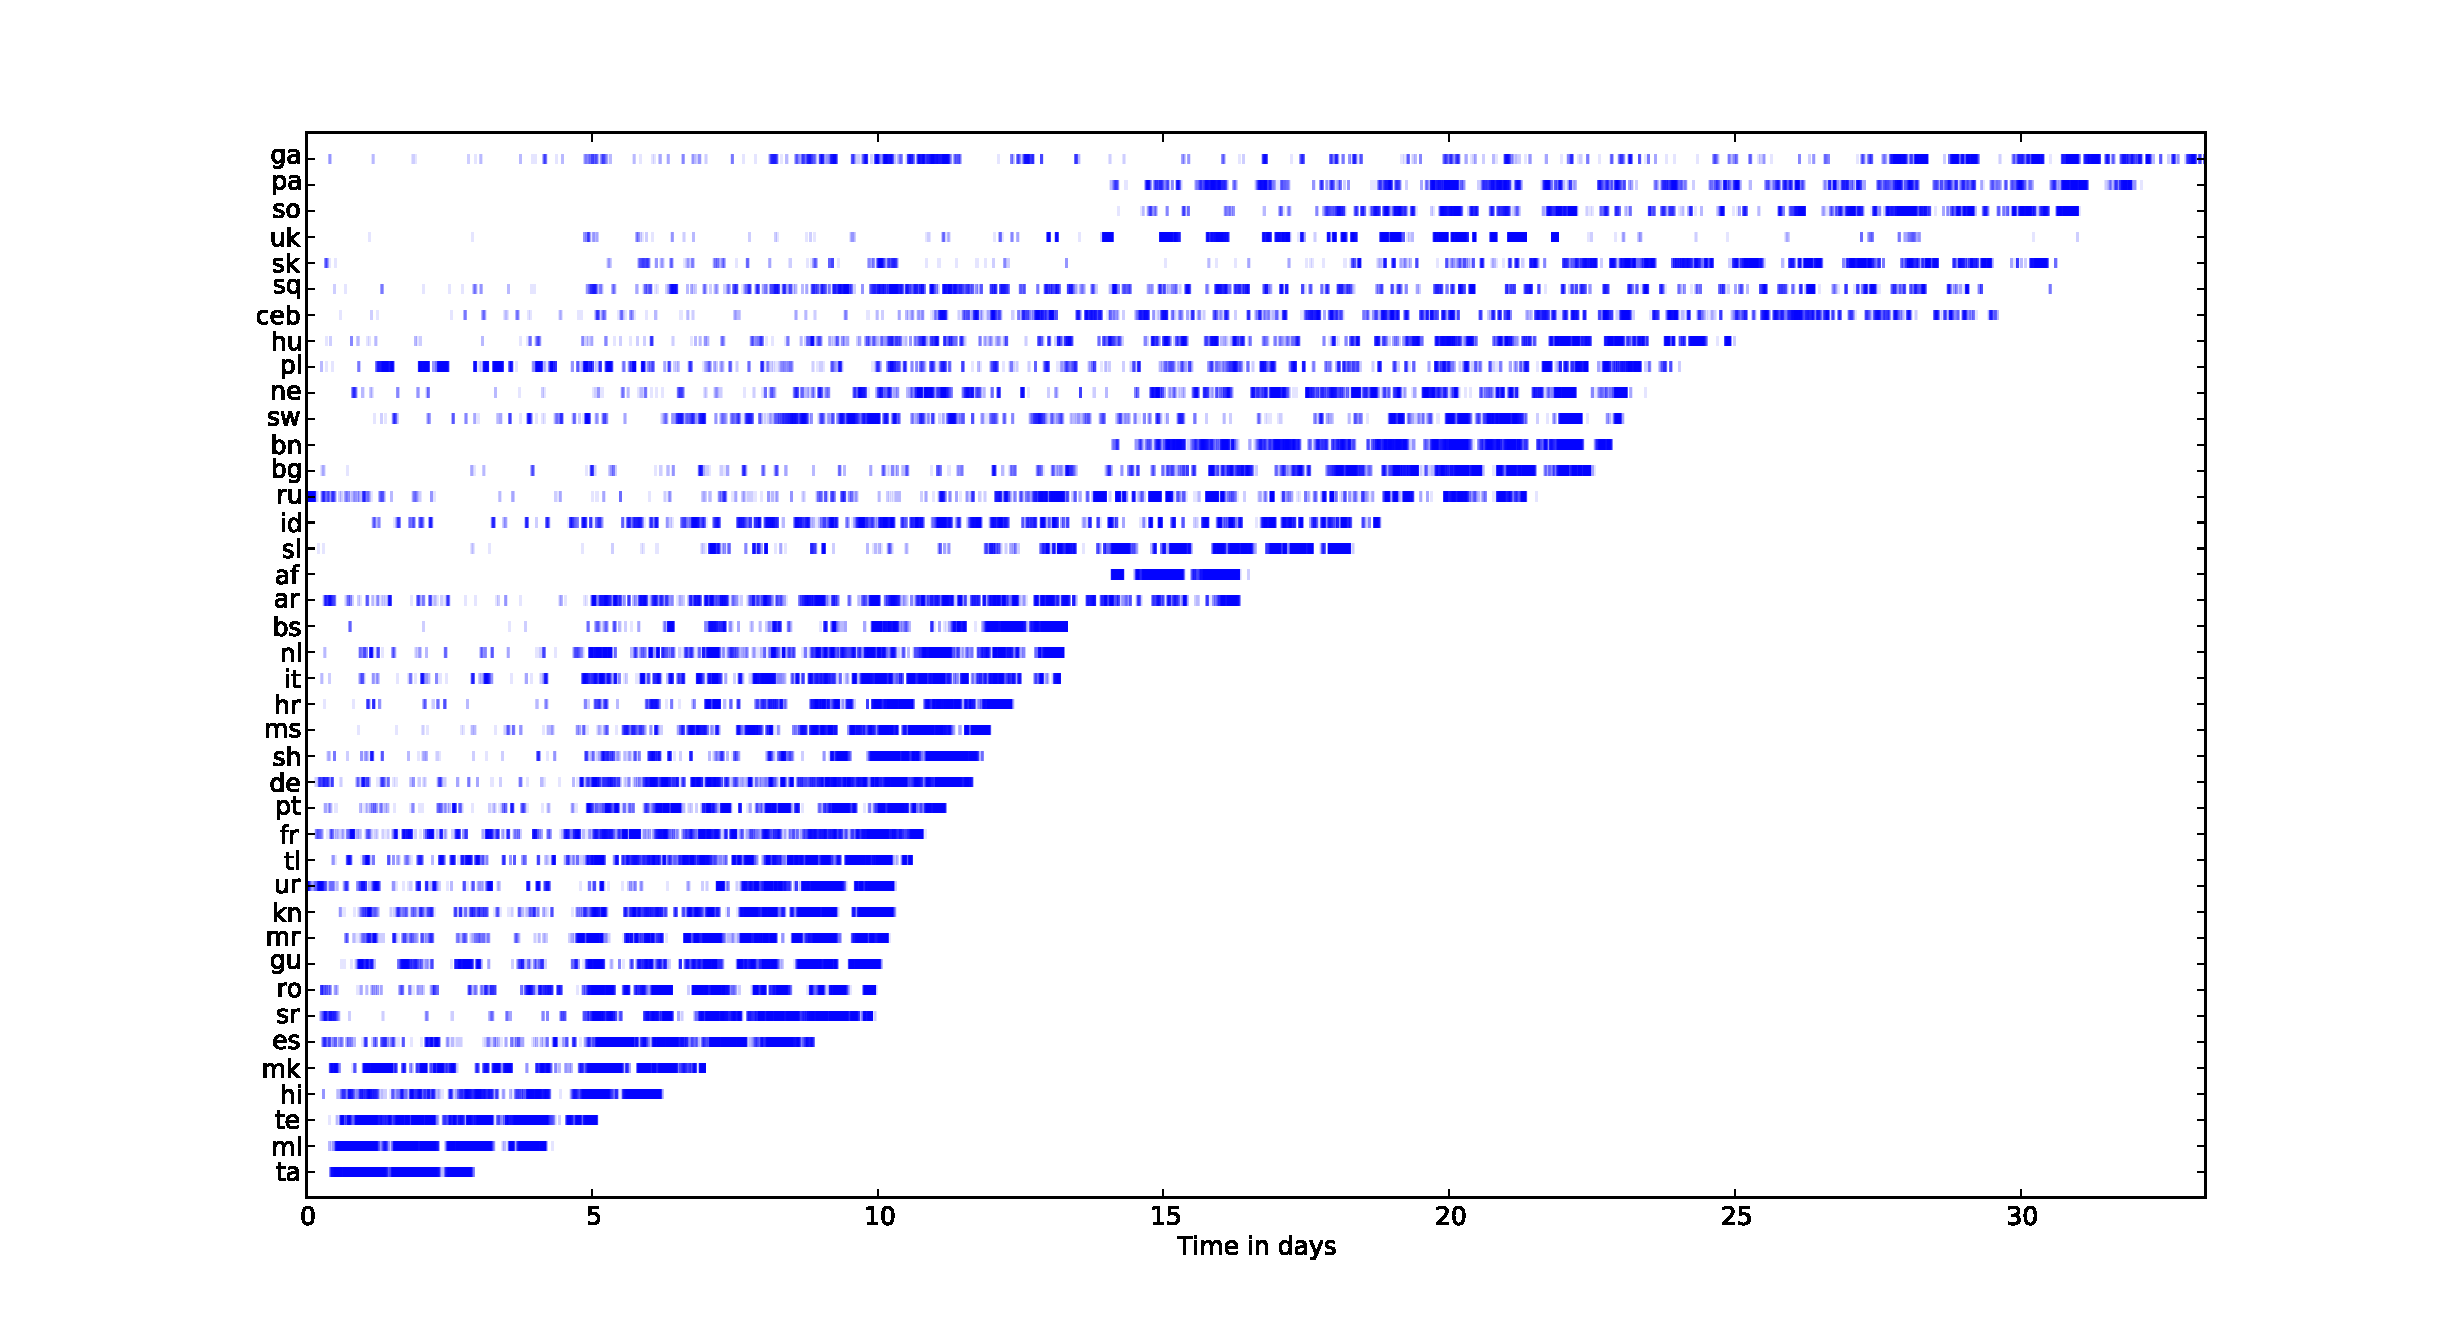
\includegraphics[height=\linewidth,angle=270]{figures/completetime}
%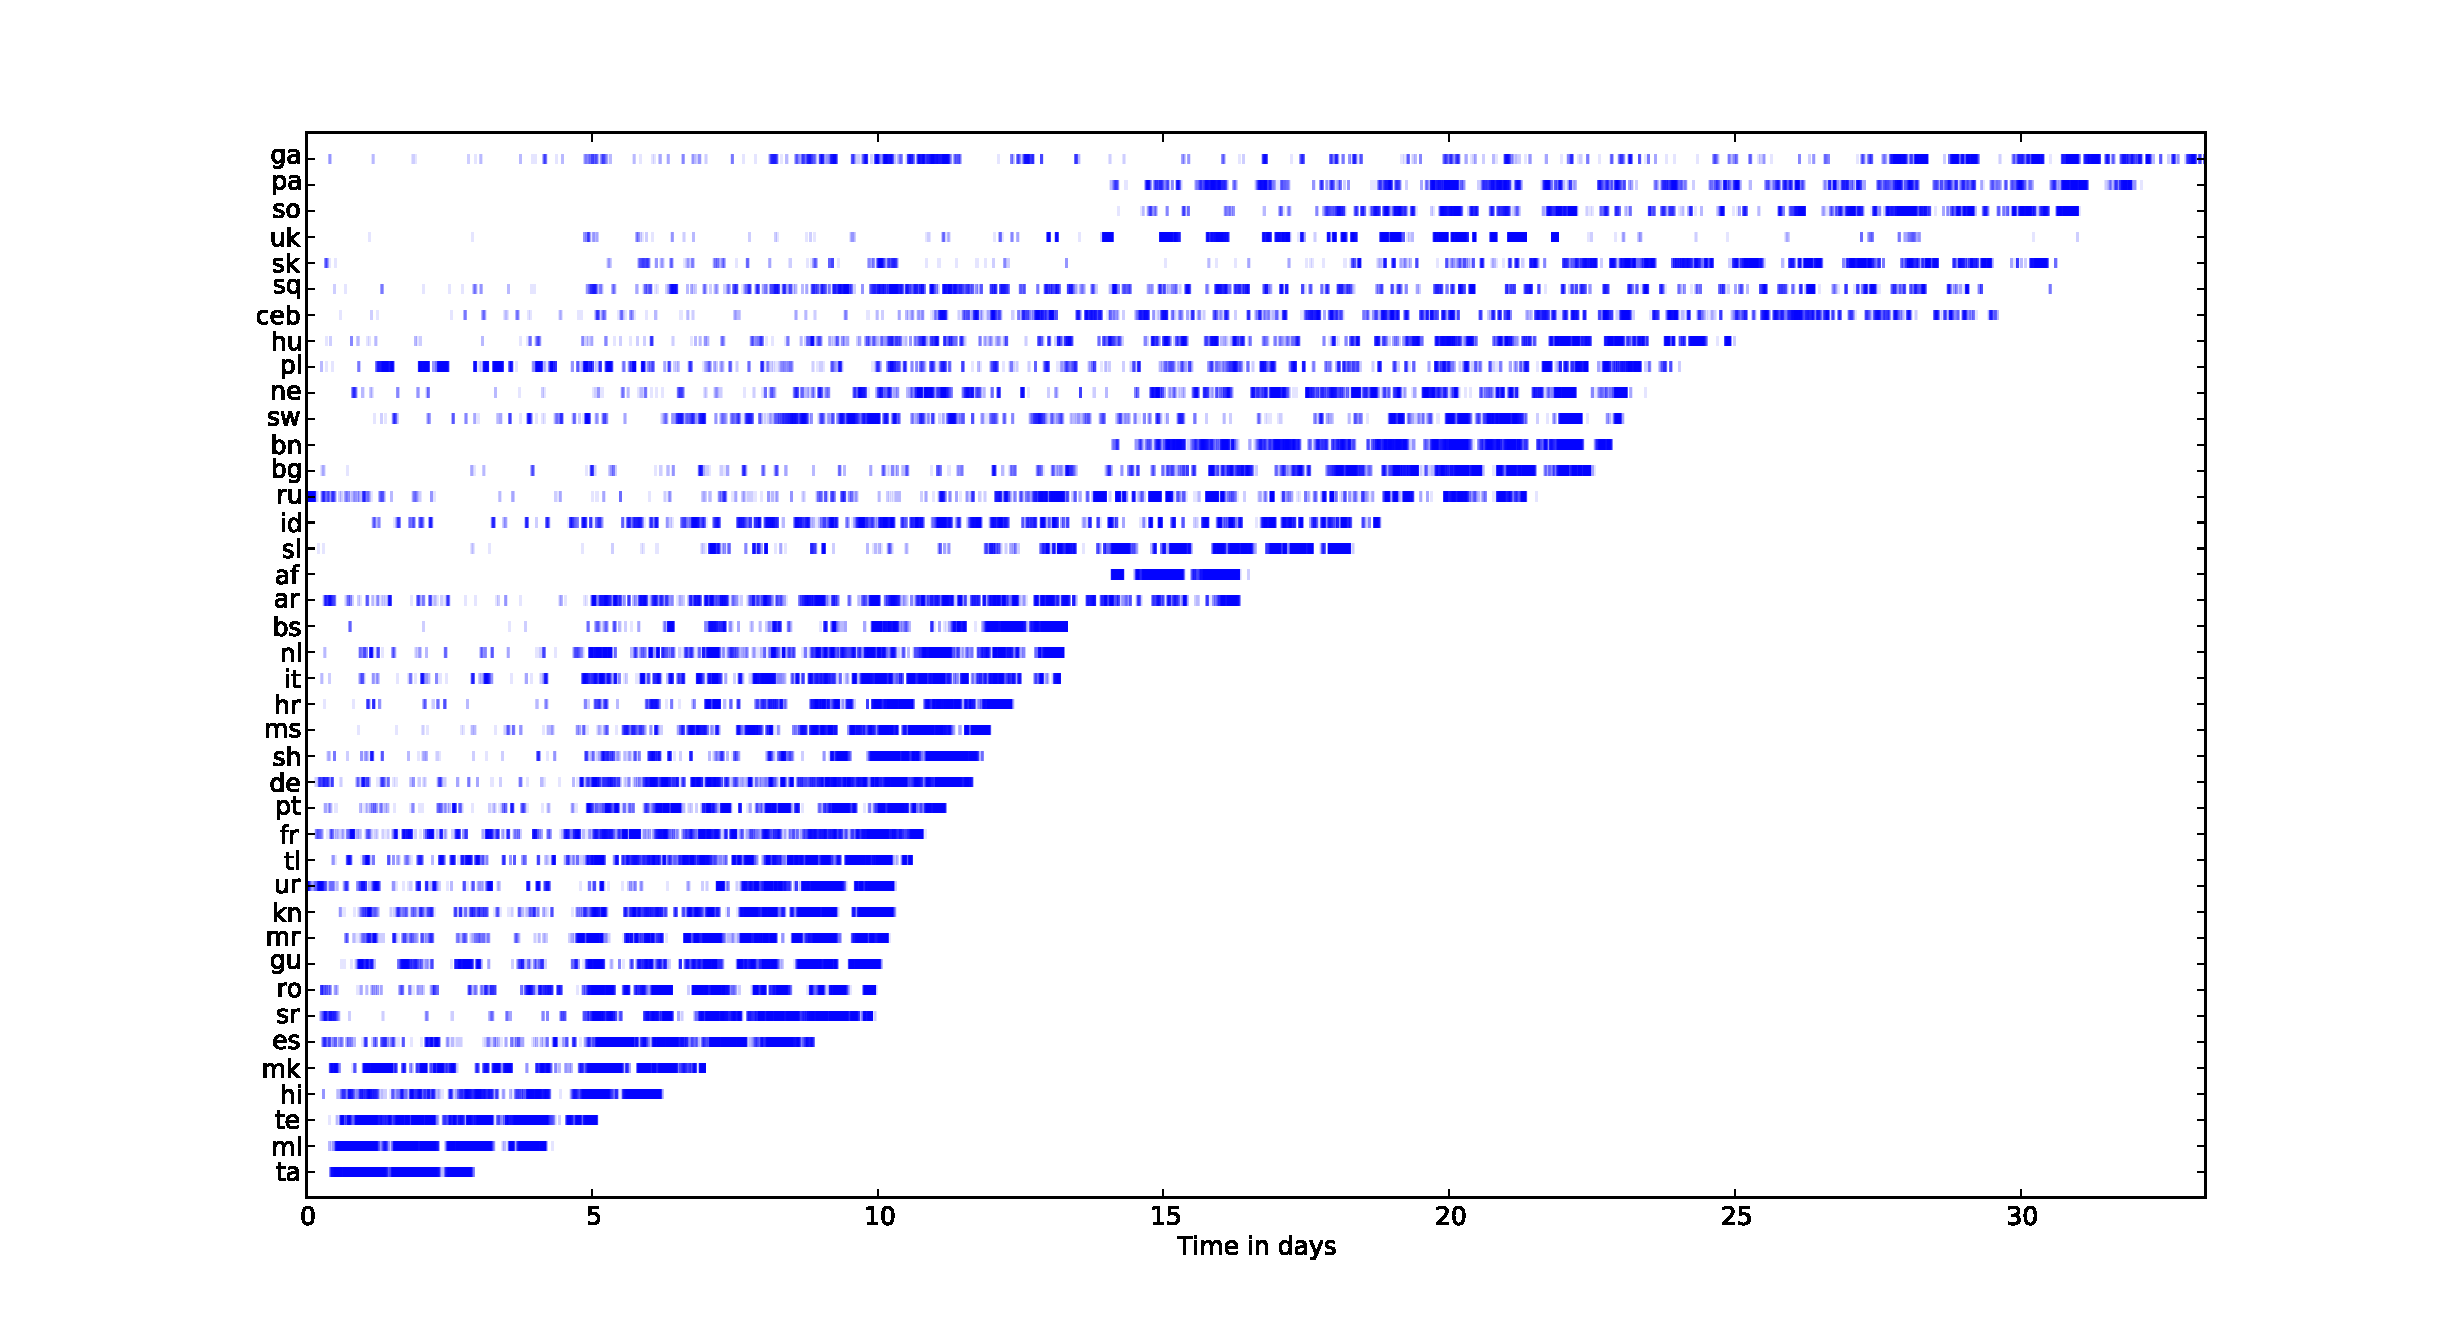
\includegraphics[width=\linewidth]{figures/completetime}
\caption{Days to complete the translation HITs for 40 of the languages. Tick marks represent the completion of individual assignments. }
\label{completion-time}
\end{figure}
%%%%%%%%%%%%%%%%%%%%%%%%%%%%%%%%%%%%%%%

\paragraph{Gold standard translations} 
A set of gold standard translations were automatically harvested from Wikipedia  for every language to use as embedded controls. We used Wikipedia's inter-language links to pair titles of English articles with their corresponding foreign article's title.  To get a more translatable set of pairs, we excluded any pairs where: (1) the English word was not present in the WordNet ontology  \cite{miller1995wordnet}, (2) either article title was longer than a single word, (3) the English Wikipedia page was a subcategory of person or place, or (4) the English and the foreign titles were identical or a substring of the other.

\paragraph{Manual evaluation of non-identical translations}
We counted all translations that exactly matched the gold standard translation as correct.  For non-exact matches we created a second-pass quality assurance HIT.  
Turkers were shown a pair of English words, one of which was a Turker's translation of the foreign word used for quality control, and the other of which was the gold-standard translation of the foreign word. Evaluators were asked whether the two words had the same meaning, and chose between three answers: `Yes', `No', or `Related but not synonymous.'  Examples of meaning equivalent pairs include: $<${\it petroglyphs, rock paintings}$>$, $<${\it demo, show}$>$ and  $<${\it loam, loam: soil rich in decaying matter}$>$.  Non-meaning equivalents included: $<${\it assorted, minutes}$>$, and $<${\it major,} URL of image$>$.  Related items were things like $<${\it sky, clouds}$>$. Misspellings like $<${\it lactation, lactiation} $>$ were judged to have same meaning, and were marked as misspelled.   Three separate Turkers judged each pair, allowing majority votes for difficult cases. 


We checked Turkers who were working on this task by embedding pairs of words which were either known to be synonyms (drawn from WordNet) or  unrelated (randomly chosen from a corpus). 
Automating approval/rejections for the second-pass evaluation allowed the whole pipeline to be run automatically.  Caching judgments meant that we ultimately needed only 
20,952 synonym tasks to judge all of the submitted translations (a total of  74,572 non-matching word pairs).  These were completed by an additional 1,005 workers.  Each of these assignments included 10 word pairs and paid \$0.10.

\begin{figure}[t]
  \centering
  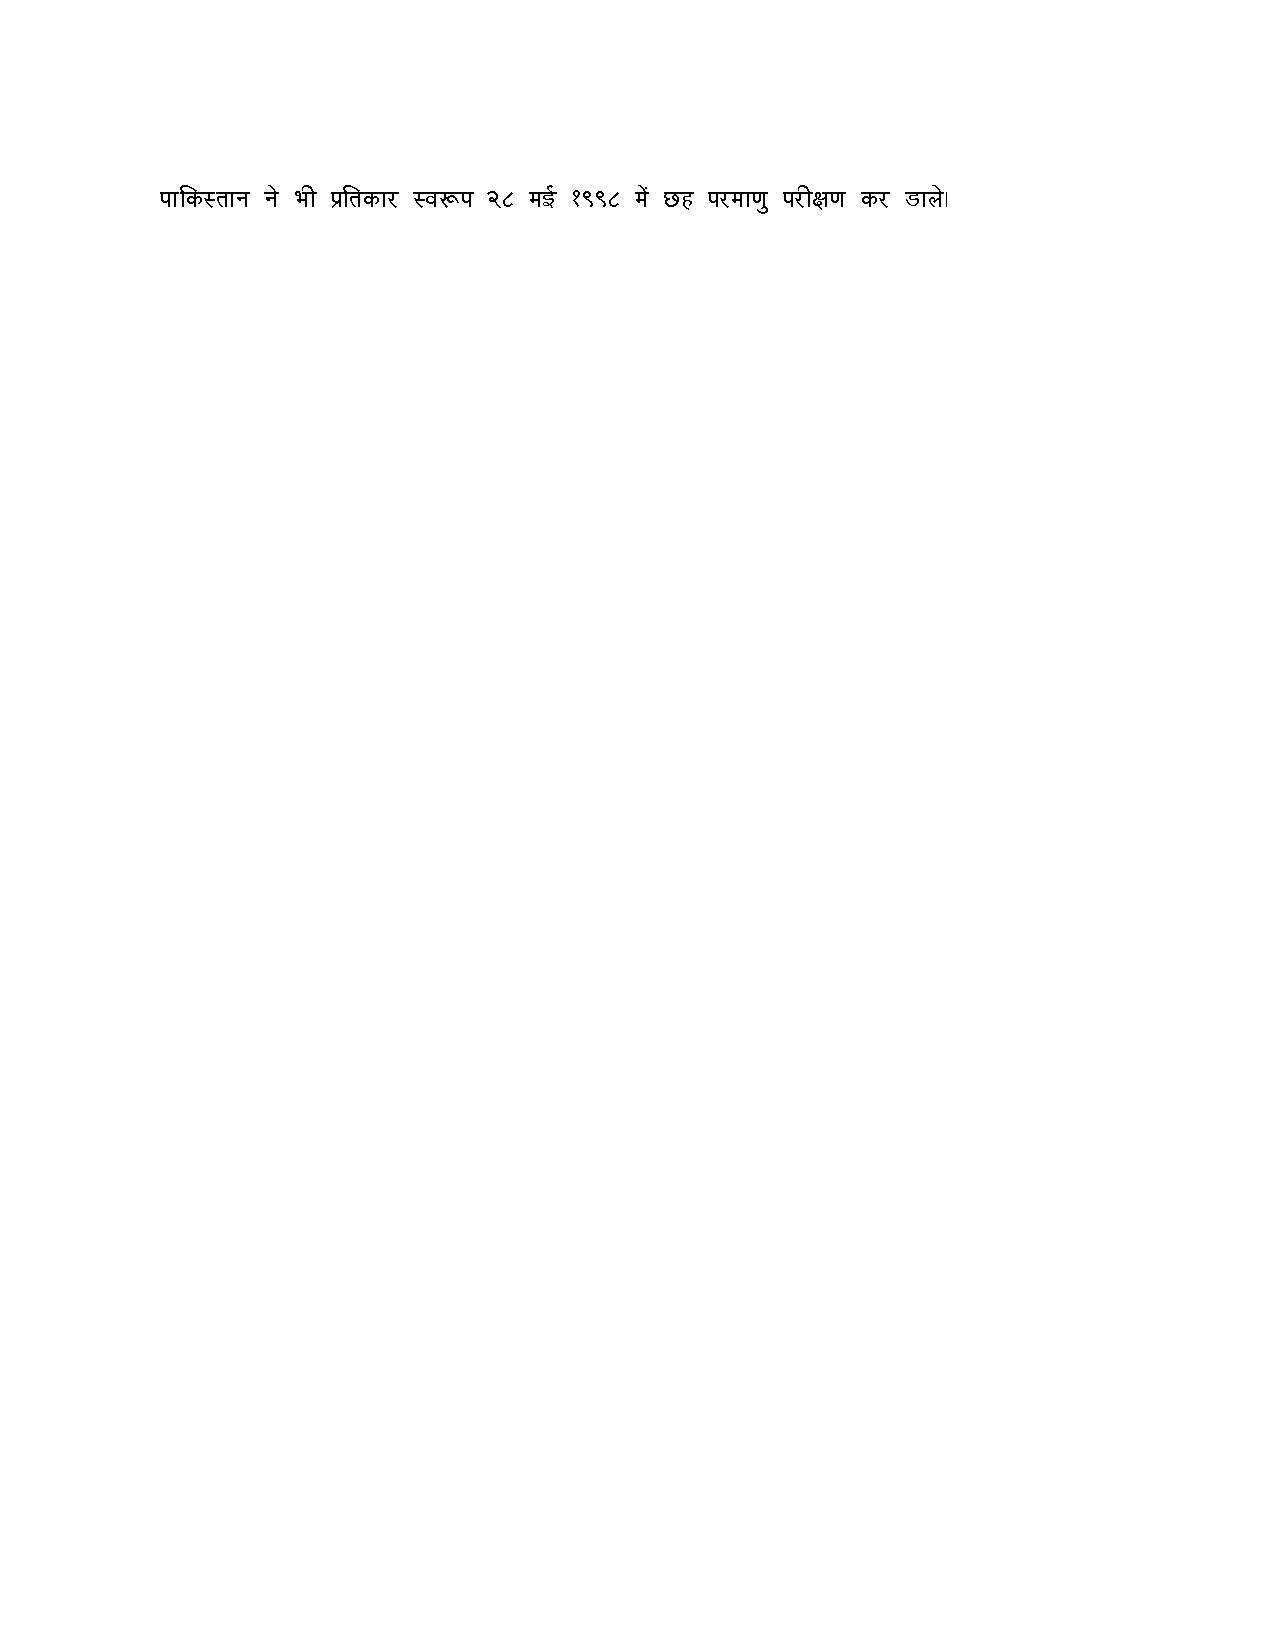
\includegraphics[width=1.05\linewidth]{figures/hindi.pdf}
  \footnotesize
  \begin{tabular}{p{\linewidth}}
    \hline
In retribution pakistan also did six nuclear tests on 28 may 1998.\\
On 28 May Pakistan also conducted six nuclear tests as an act of redressal.\\
Retaliating on this 'Pakistan' conducted Six(6) Nuclear Tests on 28 May, 1998.\\
pakistan also did 6 nuclear test in retribution on 28 may, 1998 \\ \\
  \end{tabular}
  \normalsize
  \caption{An example of the Turkers' translations of a Hindi sentence. The translations are unedited and contain fixable spelling, capitalization and grammatical errors.}
  \label{figure:variance}
\end{figure}



%%%%%%%%%%%%%%% HITLANG QUALITY BAR %%%%%%%%%%%
\begin{figure*}[h]
\begin{center}
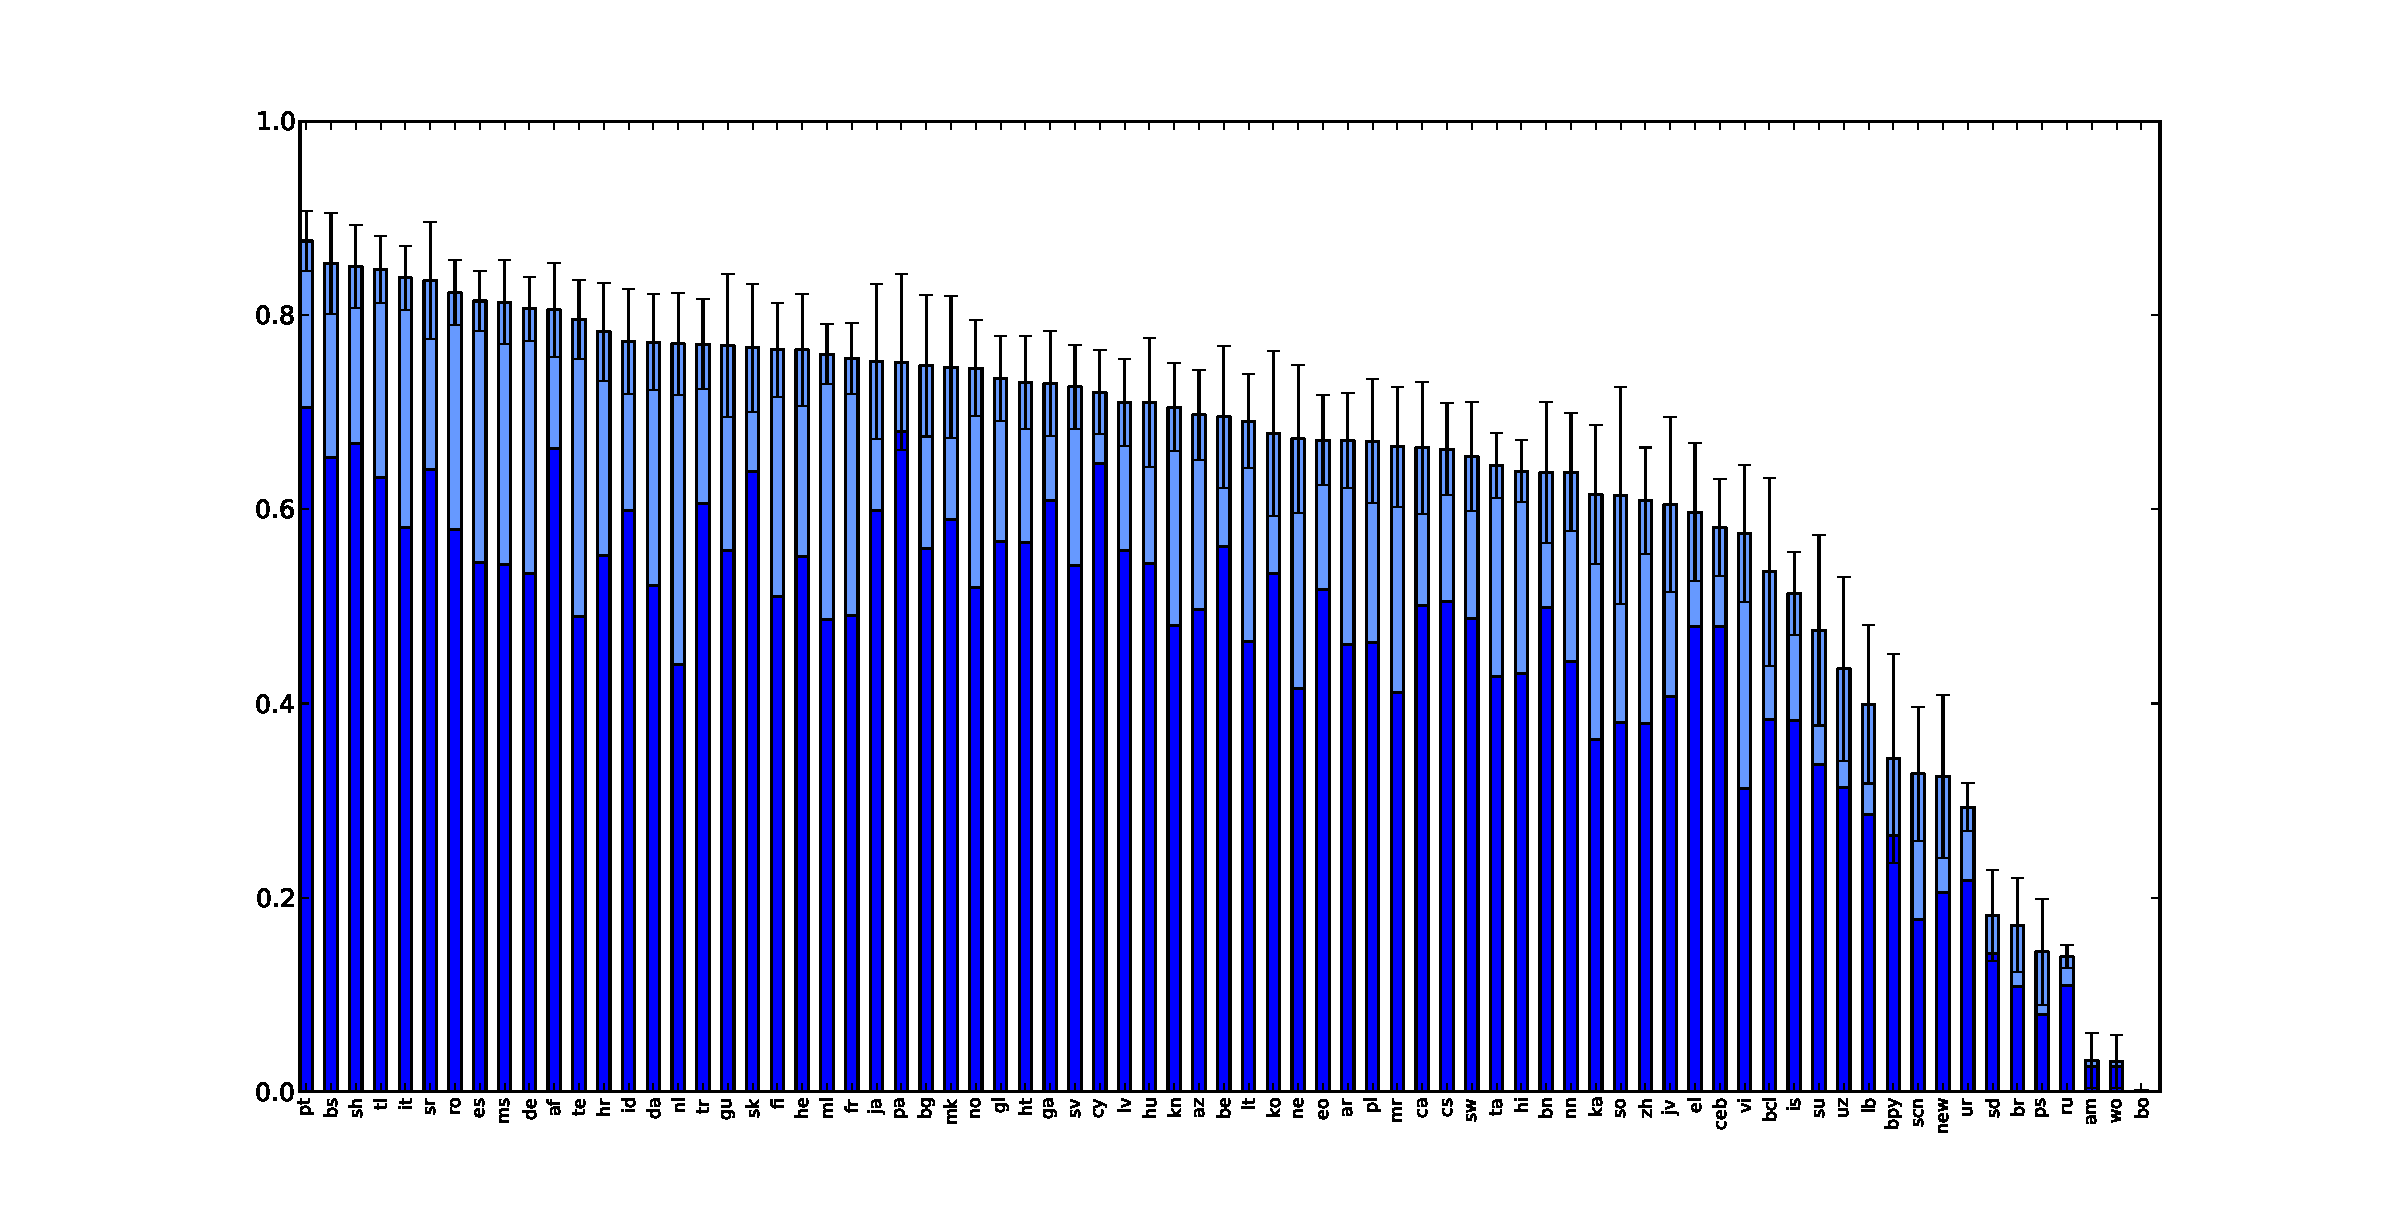
\includegraphics[width=.9\linewidth]{figures/quality_bar.pdf}
\caption{Translation quality for languages with at least 50 Turkers. The dark blue bars indicate the proportion of translations which exactly matched gold standard translations, and light blue indicate translations which were judged to be correct synonyms. Error bars show the 95\% confidence intervals for each language.}
\label{hitlangqual} 
\end{center}
\end{figure*}
%%%%%%%%%%%%%%%%%%%%%%%%%%%%%%%%%%%%%%%%%%%%%%%%%%%%%%%%

\paragraph{Full sentence translations}
To demonstrate the feasibility of using crowdsourcing to create multilingual technologies, we hire Turkers to construct bilingual parallel corpora from scratch for six Indian languages.  \newcite{Germann2001} attempted to build a Tamil-English translation system from scratch by hiring professional translators, but found the cost prohibitive. We created parallel corpora by translating the 100 most viewed Wikipedia pages in Bengali, Malyalam, Hindi, Tamil, Telugu, and Urdu into English.  We collected four translations from different Turkers for each source sentence.  

%Embedding gold-standard translations into our full-sentence translation HITs was problematic for two reasons: (1) few public bilingual parallel corpora exist for our chosen languages, and (2) Google could have trained its translation system on them already, resulting in high quality translations when Turkers used MT to translate the gold standard sentences. and it could not be mined in a straight-forward way as in the single word case, we were unable to embed controls into our HITs. 
Workers were paid \$0.70 per HIT to translate 10 sentences.  
 We  accepted or rejected translations based on a manual review of each worker's submissions, which included a comparison of the translations to a monotonic gloss (produced with a dictionary), and metadata such as the amount of time the worker took to complete the HIT and their geographic location.

Figure~\ref{figure:variance} shows an example of the translations we obtained. The lack of a professionally translated reference sentences prevented us from doing a systematic comparison between the quality of profession and non-professional translations as  \newcite{zaidan-callisonburch:2011:ACL-HLT2011a} did. Instead we evaluate the quality of the data by using it to train SMT systems. We present results in section \ref{sec:data-analysis}.



\section{Measuring Translation Quality}

For single word translations, we calculate the quality of translations on the level of individual assignments and aggregated over workers and languages.  We define an assignment's quality as the proportion of controls that are correct in a given assignment, where correct means exactly correct or judged to be synonymous.
\begin{align}	
	\text{Quality}(a_i) = \frac{1}{k_i}\sum\limits_{j=1}^{k_i}\mathbf{\delta}(tr_{ij} \in \texttt{syns[$g_j$]})
\end{align}	
where $a_i$ is the $i^{th}$ assignment, $k_i$ is the number of controls in $a_i$, $tr_{ij}$ is the Turker's provided translation of control word $j$ in assignment $i$, $g_j$ is the gold standard translation of control word $j$, \texttt{syns[$g_j$]} is the set of words judged to be synonymous with $g_j$ and includes $g_j$, and $\mathbf{\delta}(x)$ is Kronecker's delta and takes value 1 when $x$ is true. 
Most assignments had two known words embedded, so most assignments had scores of either 0, 0.5, or 1. 


Since computing overall quality for a language as the average assignment quality score is biased towards a small number of highly active Turkers, we instead report language quality scores as the average per-Turker quality, where a Turker's quality is  the average quality of all the assignments that she completed:
\begin{align}	
	\text{Quality}(t_i) = \frac{\sum_{a_j \in \texttt{assigns[$i$]}}\text{Quality}(a_j)}{\mid \texttt{assigns[$i$]} \mid}
\end{align}	
where \texttt{assigns[$i$]} is the assignments completed by Turker $i$, and Quality($a$) is as above.

Quality for a language is then given by
\begin{align}	
	\text{Quality}(l_i) = \frac{\sum_{t_j \in \texttt{turkers[$i$]}}\text{Quality}(t_j)}{\mid \texttt{turkers[$i$]} \mid}
\end{align}	
When a Turker completed assignments in more than one language, their quality was computed separately for each language. Figure \ref{hitlangqual} shows the translation quality for languages with contributions from at least 50 workers.  


\paragraph{Cheating using machine translation}


One obvious way for workers to cheat is to use available online translation tools. Although we followed best practices to deter copying-and-pasting into online MT systems  by  rendering words and sentences as images \cite{zaidan-callisonburch:2011:ACL-HLT2011a}, this strategy does not prevent workers from typing the words into an MT system if they are able to type in the language's script. 

To identify and remove workers who appeared to be cheating by using Google Translate, we calculated each worker's overlap with the Google translations. We used Google to translate all 10,000 words for the 51 foreign languages that Google Translate covered at the time of the study. We measured the percent of workers' translations that exactly matched the translation returned from Google. 

%Results are show in Figure \ref{googlematch}. Assignments averaged around 42\% overlap with GoogleTranslate.  Languages with non-Latin scripts (such as the Arabic script, Chinese characters or the Telugu alphabet) have lower overlap with Google,  suggesting that it is easier for Turkers to cheat for languages written in the Latin alphabet. 

%%%%%%%%%%%%%%% GOOGLE OVERLAP BAR %%%%%%%%%%%
%\begin{figure}[h]
%\begin{center}
%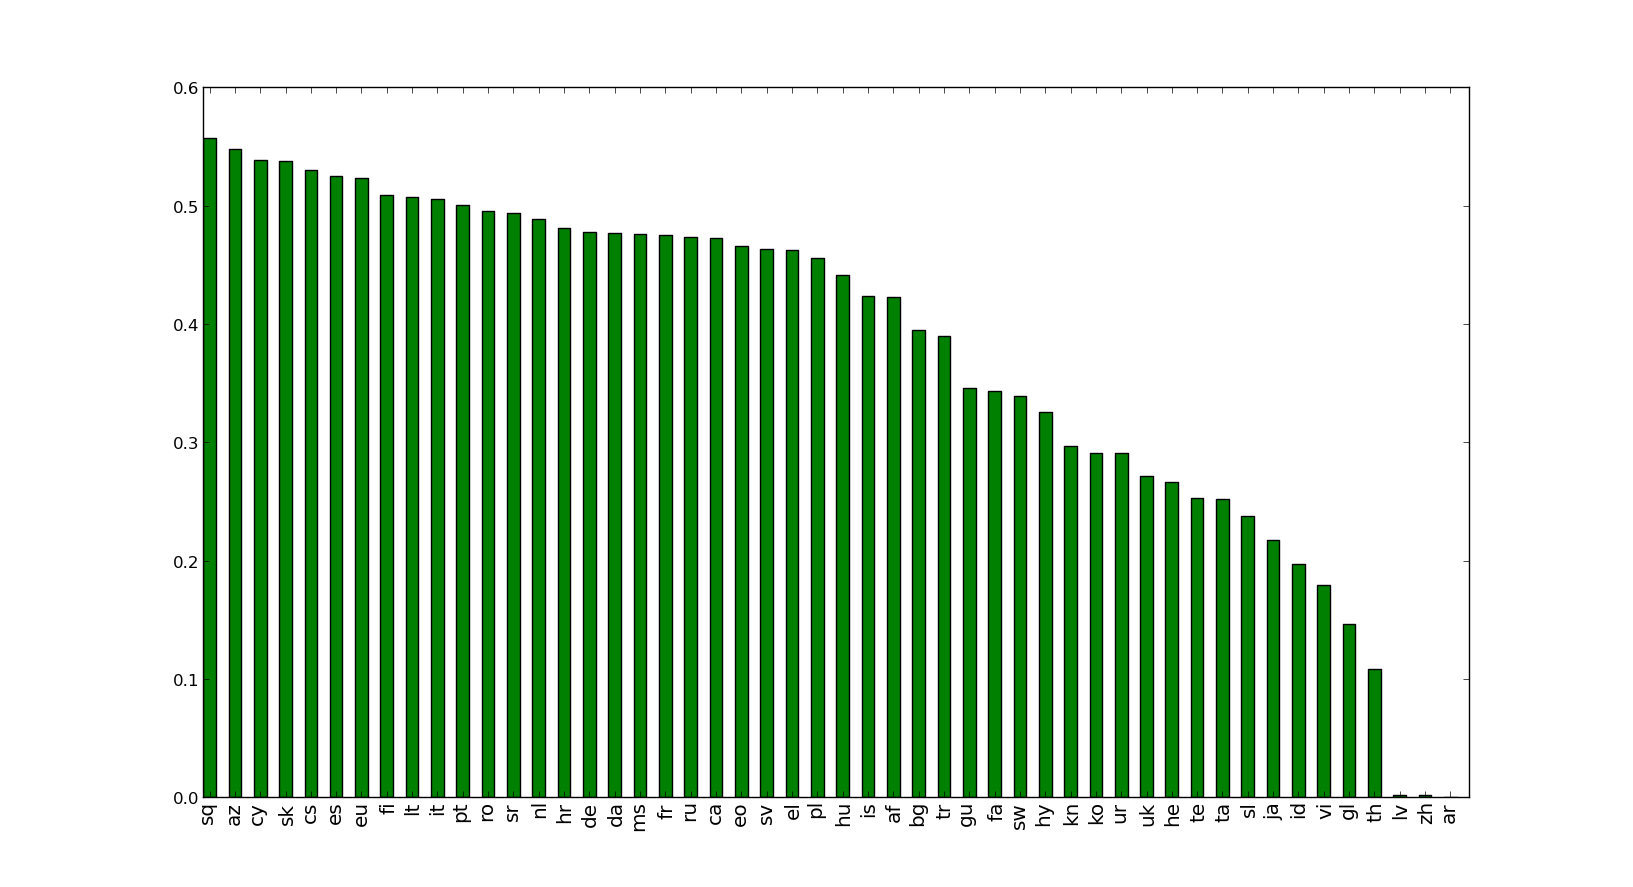
\includegraphics[width=1\linewidth]{figures/google_bar.pdf}
%\caption{Average proportion of Turker translations matching GoogleTranslate, per assignment. Overall average overlap was 0.37.}
%\label{googlematch} 
%\end{center}
%\end{figure}
%%%%%%%%%%%%%%%%%%%%%%%%%%%%%%%%%%%%%%%%%%%%%%%%%%%%%%%%


\begin{figure}[h!]
\centering
\begin{subfigure}[b]{\linewidth}
%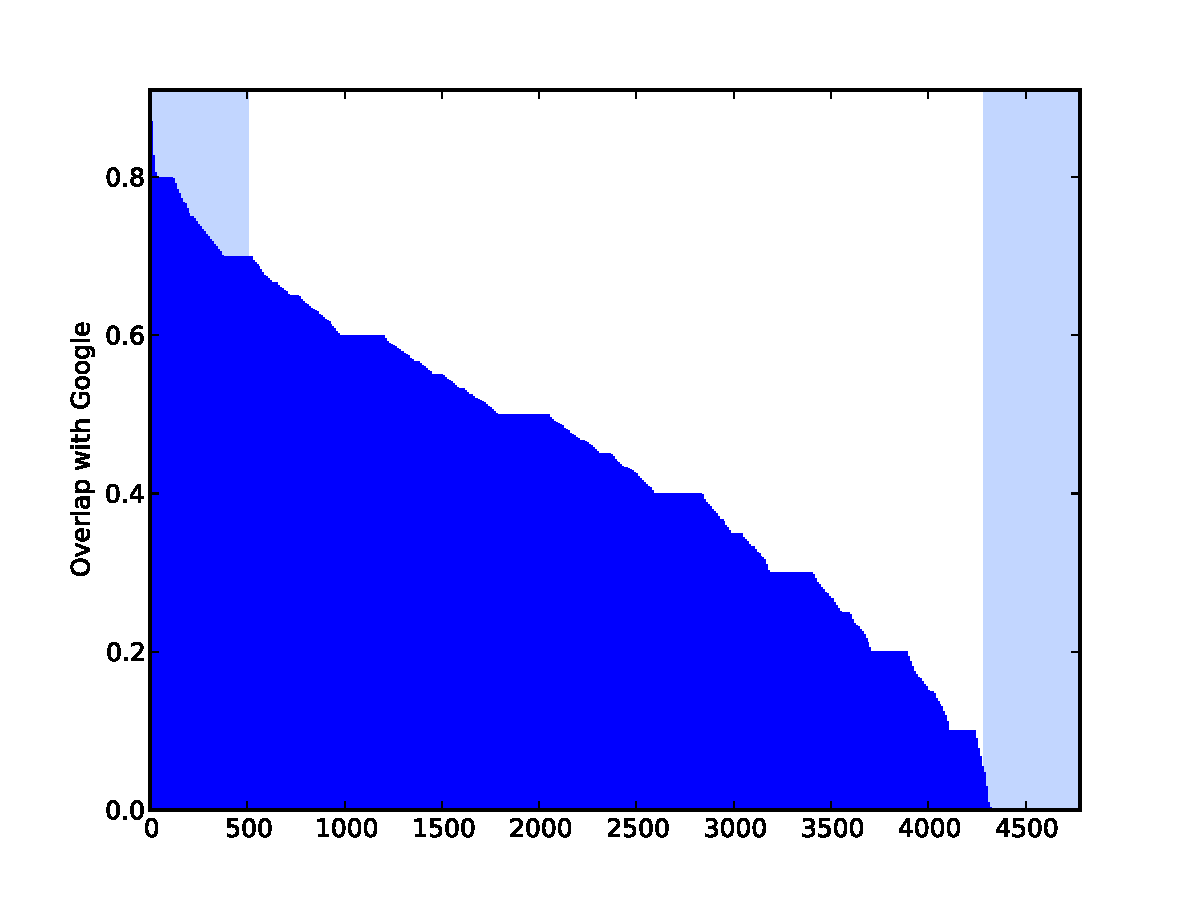
\includegraphics[width=\textwidth]{figures/turker-googmatch-distribution.pdf}
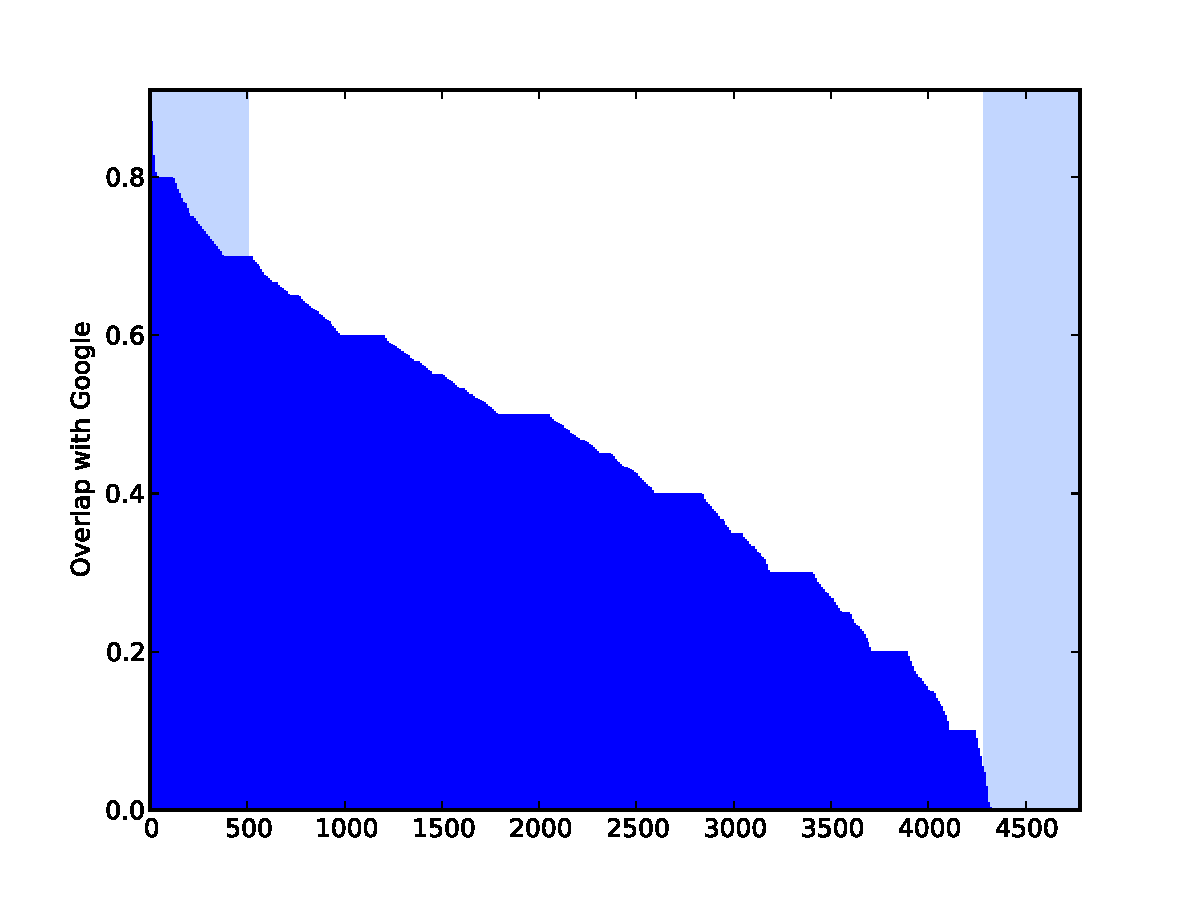
\includegraphics[width=\linewidth]{figures/turker-googmatch-distribution.pdf}
\caption{Individual workers' overlap with Google Translate. We removed the 500 workers with the highest overlap (shaded region on the left) from our analyses, as it is reasonable to assume these workers are cheating by submitting translations from Google. Workers with no overlap (shaded region on the right) are also likely to be cheating, e.g. by submitting random text. }
%, and we target these workers through our embedded quality controls.}                
\label{dist}
\end{subfigure}
\begin{subfigure}[b]{\linewidth}
%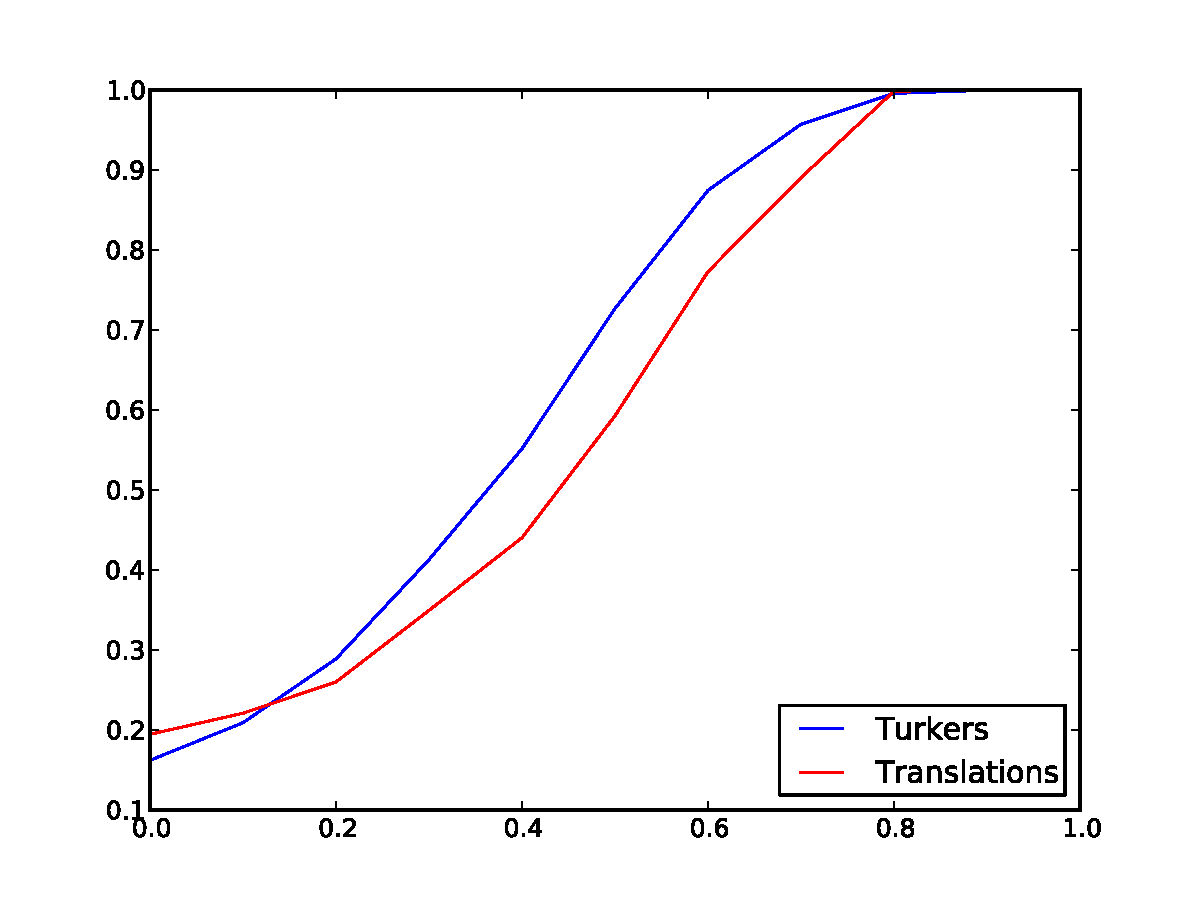
\includegraphics[width=\textwidth]{figures/google-cdf-googlangs.pdf}
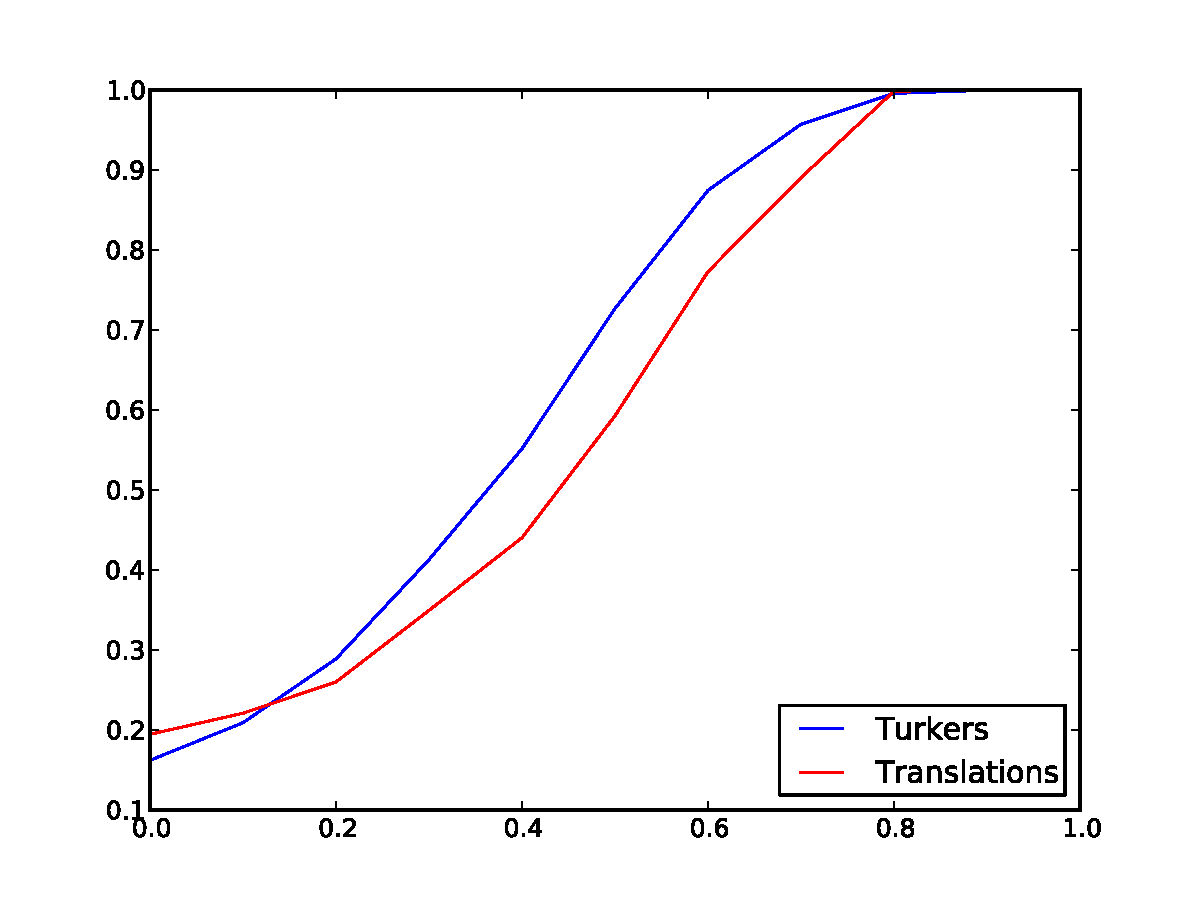
\includegraphics[width=\linewidth]{figures/google-cdf-googlangs.pdf}
\caption{Cumulative distribution of overlap with Google translate for workers and translations. We see that eliminating all workers with \textgreater 70\% overlap with google translate still preserves 90\% of translations and \textgreater 90\% of workers.}
\label{cdf}
\end{subfigure}
\caption{}\label{cheaters}
\end{figure}

%We found that while overall overlap is high (the average worker's overlap was 41\%), it is not consistently high across all workers. 
Figure \ref{dist} shows overlap between Turkers's translations and Google Translate.  When overlap is high, it seems likely that those Turkers are cheating.  It is also reasonable to assume that honest workers will overlap with Google some amount of the time as Google's translations are usually accurate. We divide the workers into three groups: those with very high overlap with Google (likely cheating by using Google to translate words), those with reasonable overlap, and those with no overlap (likely cheating by other means, for instance, by submitting random text).  
 
Our gold-standard controls are designed to identify workers that fall into the third group (those who are spamming or providing useless translations), but they will not effectively flag workers who are cheating with Google Translate. We therefore remove the 500 Turkers with the highest overlap with Google. This equates to removing all workers with greater than 70\% overlap. Figure \ref{cdf} shows that removing workers at or above the 70\% threshold retains 90\% of the collected translations and over 90\% of the workers.

Quality scores reported throughout the paper reflect only translations from Turkers whose overlap with Google falls below this 70\% threshold.



%%%%%%%%%%%%%%% TURKER QUAL SUMMARY TABLE %%%%%%%%%%%
\begin{table*}
\scriptsize
\begin{center}
\begin{tabular}{lllll}
\hline\hline
&\multicolumn{2}{c}{Avg. Turker quality (\# Ts)}&Primary locations&Primary locations\\
&In region&Out of region&of Turkers in region&of Turkers out of region\\
\hline\hline
Hindi & 0.63 (296) & \textbf{0.69} (7) & India (284) UAE (5) UK (3)  & Saudi Arabia (2) Russia (1) Oman (1) \\
Tamil & \textbf{0.65} (273) ** & 0.25 (2) & India (266) US (3) Canada (2)  & Tunisia (1) Egypt (1)  \\
Malayalam & 0.76 (234) & \textbf{0.83} (2) & India (223) UAE (6) US (3)  & Saudi Arabia (1) Maldives (1) \\
Spanish & 0.81 (191) & \textbf{0.84} (18) & US (122) Mexico (16) Spain (14)  & India (15) New Zealand (1) Brazil (1) \\
French & 0.75 (170) & \textbf{0.82} (11) & India (62) US (45) France (23)  & Greece (2) Netherlands (1) Japan (1) \\
Chinese & \textbf{0.60} (116) & 0.55 (21) & US (75) Singapore (13) China (9)  & Hong Kong (6) Australia (3) Germany (2)  \\
German & \textbf{0.82} (91) & 0.77 (41) & Germany (48) US (25) Austria (7)  & India (34) Netherlands (1) Greece (1)  \\
Italian & \textbf{0.86} (90) * & 0.80 (42) & Italy (42) US (29) Romania (7)  & India (33) Ireland (2) Spain (2)  \\
Amharic & \textbf{0.14} (16) ** & 0.01 (99) & US (14) Ethiopia (2)  & India (70) Georgia (9) Macedonia (5)  \\
Kannada & 0.70 (105) & NA (0) & India (105)  & \\
Arabic & \textbf{0.74} (60) ** & 0.60 (45) & Egypt (19) Jordan (16) Morocco (9)  & US (19) India (11) Canada (3)  \\
Sindhi & \textbf{0.19} (96) & 0.06 (9) & India (58) Pakistan (37) US (1)  & Macedonia (4) Georgia (2) Indonesia (2)  \\
Portuguese & 0.87 (101) & \textbf{0.96} (3) & Brazil (44) Portugal (31) US (15)  & Romania (1) Japan (1) Israel (1) \\
Turkish & 0.76 (76) & \textbf{0.80} (27) & Turkey (38) US (18) Macedonia (8)  & India (19) Pakistan (4) Taiwan (1) \\
Telugu & \textbf{0.80} (102) & 0.50 (1) & India (98) US (3) UAE (1)  & Saudi Arabia (1)  \\
Irish & \textbf{0.74} (54) & 0.71 (47) & US (39) Ireland (13) UK (2)  & India (36) Romania (5) Macedonia (2)  \\
Swedish & \textbf{0.73} (54) & 0.71 (45) & US (25) Sweden (22) Finland (3)  & India (23) Macedonia (6) Croatia (2)  \\
Czech & \textbf{0.71} (45) * & 0.61 (50) & US (17) Czech Republic (14) Serbia (5)  & Macedonia (22) India (10) UK (5)  \\
Russian & \textbf{0.15} (67) * & 0.12 (27) & US (36) Moldova (7) Russia (6)  & India (14) Macedonia (4) UK (3)  \\
Breton & 0.17 (3) & \textbf{0.18} (89) & US (3)  & India (83) Macedonia (2) China (1) \\
\hline\hline
\end{tabular}
\normalsize
\end{center}
\caption{Translation quality when partitioning the translations into two groups, one containing translations submitted by Turkers whose location is within regions that plausibly speak the foreign language, and the other containing translations from Turkers outside those regions. In general, in-region Turkers provide higher quality translations. (**) indicates differences significant at p=0.05, (*) at p=0.10.} \label{region-summary}
\end{table*}
%%%%%%%%%%%%%%%%%%%%%%%%%%%%%%%%%%%%%%%%%%%%%%%%%%%%%%%%

\section{Data Analysis} \label{sec:data-analysis}

We performed an analysis of our data to address the following questions:
\begin{itemize}
\item Do workers accurately represent their language abilities?  Should we constrain tasks by region? 
\item How quickly can we expect work to be completed in a particular language? 
%\item Are our gold standard translations valid? 
\item Can Turkers' translations be used to train MT systems? 
\item Do our dictionaries improve MT quality?
\end{itemize}



\paragraph{Language skills and location}

We measured the average quality of workers who were in countries that plausibly speak a language, versus workers from countries that did not have large speaker populations of that language.  We used the Ethnologue \cite{ethnologue} to compile the list of countries where each language is spoken.  Table \ref{region-summary} compares the average translation quality of assignments completed within the region of each language, and compares it to the quality of assignments completed outside that region. 

Our workers reported speaking 95 languages natively. US workers alone reported 61 native languages. Overall, 4,297 workers were located in a region likely to speak the language from which they were translating, and 2,778 workers were located in countries considered out of region (meaning that about a third of our 5,281 Turkers completed HITs in multiple languages). 

Table \ref{region-summary} shows the differences in translation quality when computed using in-region versus out-of-region Turkers, for the languages with the greatest number of workers.  Within region workers typically produced higher quality translations. Given the number of Indian workers on Mechanical Turk, it is unsurprising that they represent majority of out-of-region workers.  For the languages that had more than 75 out of region workers (Malay, Amharic, Icelandic, Sicilian, Wolof, and Breton), Indian workers represented at least 70\% of the out of region workers in each language.

A few languages stand out for having suspiciously strong performance by out of region workers, notably Irish and Swedish, for which out of region workers account for a near equivalent volume and quality of translations to the in region workers. This is admittedly implausible, considering the relatively small number of Irish speakers worldwide, and the very low number living in the countries in which our Turkers were based (primarily India). Such results highlight the fact that cheating using online translation resources is a real problem, and despite our best efforts to remove workers using Google Translate, some cheating is still evident. Restricting to within region workers is an effective way to reduce the prevalence of cheating. We discuss the languages which are best supported by true native speakers in section 6. 


\paragraph{Speed of translation}


Figure \ref{completion-time} gives the completion times for 40 languages.  
The 10 languages to finish in the shortest amount of time were: Tamil, Malayalam, Telugu, Hindi, Macedonian, Spanish, Serbian, Romanian, Gujarati, and Marathi. Seven of the ten fastest languages are from India, which is unsurprising given the geographic distribution of workers.  Some languages follow the pattern of having a smattering of assignments completed early, with the rate picking up later. 

Figure \ref{figure:volume-of-data-by-language} gives the throughput of the full-sentence translation task for the six Indian languages.  The fastest language was Malayalam, for which we collected half a million words of translations in just under a week.  Table \ref{table:data-size} gives the size of the data set that we created for each of these languages. 

\begin{figure}[t]
  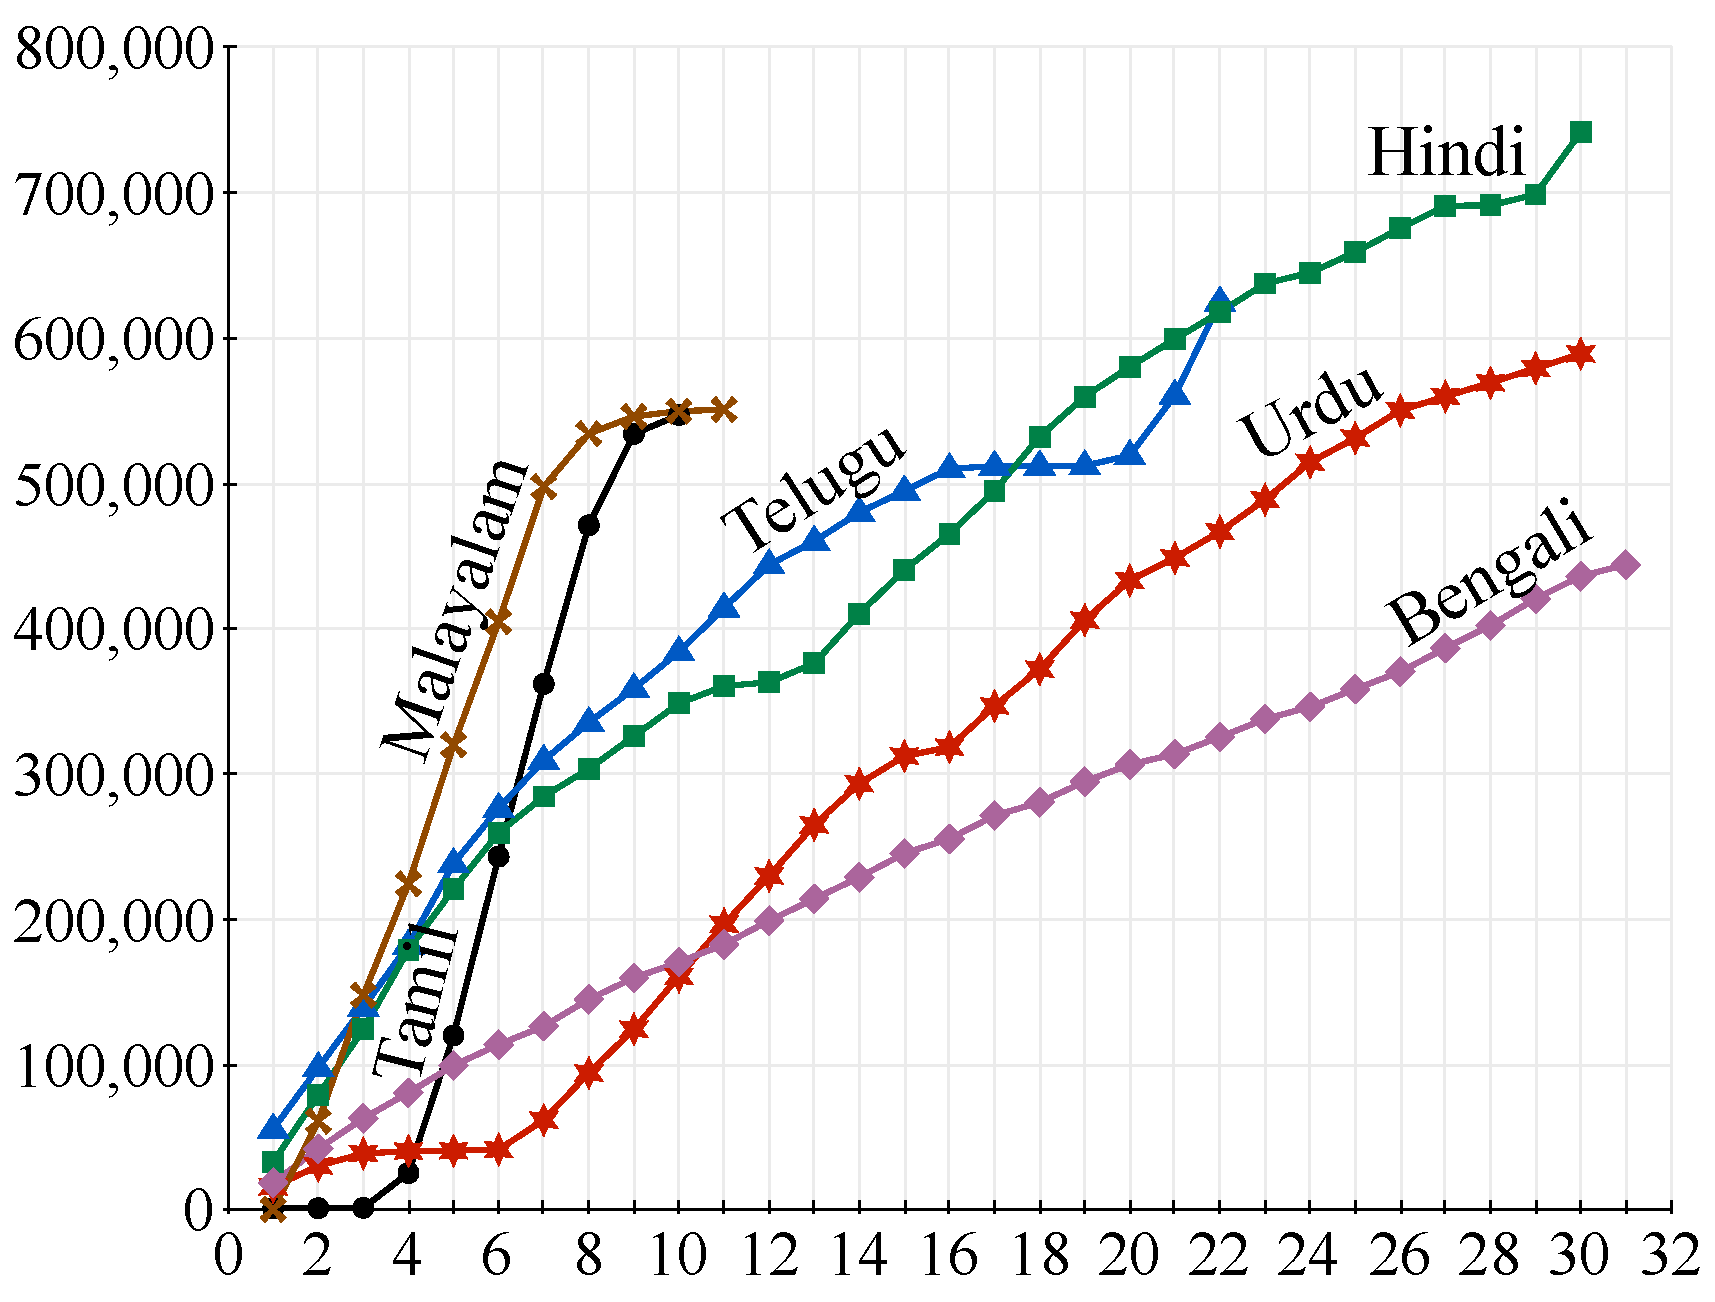
\includegraphics[width=\linewidth]{figures/volume}
  \caption{The total volume of translations (measured in English words)
    as a function of elapsed days. }
  \label{figure:volume-of-data-by-language}
\end{figure}





\begin{table}[t]
  \centering
  \small
  \begin{tabular}{l|rrr}
    		 & sentence   &  English + & dictionary  \\
    language &  pairs  & foreign words &  entries \\
    \hline\hline
    Bengali & 22k & 732k   & 22k \\
    Hindi   &  40k & 1,488k & 22k \\
    Malayalam & 32k & 863k & 23k \\
    Tamil & 38k & 916k & 25k \\
    Telugu & 46k & 1,097k & 21k \\
    Urdu & 35k & 1,356k & 20k \\
  \end{tabular}
  \caption{Size of parallel corpora and bilingual dictionaries collected for each language. }
  \label{table:data-size}
\end{table}

\begin{table}[t]
\centering
  \small
\begin{tabular}{l|cc|c}
  		  & trained on  &  bitext + & BLEU \\
  language  & bitexts alone &  dictionaries & $\Delta$ \\
  \hline\hline
  Bengali    &  12.03 & 17.29 & 5.26 \\
  Hindi      & 16.19 & 18.10 & 1.91 \\  
  Malayalam    &  6.65 & 9.72 & 3.07 \\      
  Tamil      & 8.08 & 9.66 & 1.58 \\  
  Telugu     & 11.94 & 13.70 & 1.76 \\  
  Urdu        & 19.22 & 21.98 & 2.76 \\   
\end{tabular}
\caption{BLEU scores for translating into English using bilingual parallel corpora by themselves, and with the addition of single-word dictionaries. Scores are calculated using four reference translations and represent the mean of three MERT runs.}
\label{dictionary_bleu}
\end{table}


\paragraph{Training SMT systems}
We trained statistical translation models from the parallel corpora that we created for the six Indian languages using the Joshua machine translation system \cite{post2012constructing}. Table \ref{dictionary_bleu} shows the translation performance when trained on the bitexts alone, and when incorporating the bilingual dictionaries created in our earlier HIT. The scores reflect the performance when tested on held out sentences from the training data. Adding the dictionaries to the training set produces consistent performance gains, ranging from 1 to 5 BLEU points. This represents a substantial improvement. It is worth noting, however, that while the source documents for the full sentences used for testing were kept disjoint from those used for training, there is overlap between the source materials for the dictionaries and those from the test set, since both the dictionaries and the bitext source sentences were drawn from Wikipedia. 

%Unfortunately, we do not have professionally translated data against which to compare the resulting performances, but we find the outcomes encouraging as an indication of the potential of Turkers to provide high quality translations.

%\paragraph{Validation of controls} 
%Higher overlap with Google Translate corresponds slightly to higher quality scores (Pearson $\rho$ = 0.27), suggesting that some control translations have already been indexed by Google. We therefore investigated the validity of our use of Wikipedia inter-language links as gold standard translations.
%
%As an extrinsic measure of translation quality, we measure the proportion of $<${\it word, translation}$>$ pairs received from Mechanical Turk which appear in external dictionaries.  We had external bilingual dictionaries for 24 of the 100 languages examined in this study.\footnote{The bilingual dictionaries were between English and az, bg, bn, bs, cy, es, fa, hi, id, lv, ms, ne, pl, ro, ru, sk, so, sq, sr, ta, tr, UK, ur, and uz. }  We used each of these bilingual dictionaries to compute language-level quality scores, using the dictionary's translation as a gold standard translation for any of the 10,000 foreign words in our study.  In some cases, the overlap of words was low, since dictionaries list root forms of words and we translated inflected forms.  
%
%We ranked the 24 languages based on their translation quality scores according to the external dictionaries, and calculated correlation when compared to the ranking produced by our gold standard control.  The Pearson correlation was $\rho=0.53$.  We computed a correlation coefficient of $\rho=0.37$ for ranking of the translation quality of individual Turkers using the two sources of reference translations.    
%
%Given the strong positive correlation, we are satisfied that the trends reported in this paper hold when using either our gold standard translations or external bilingual dictionaries. 



%%%%%%%%%%%%%%%%%%%%%%%%%%
\begin{table}
\centering
\footnotesize
%\small
\begin{tabular}{|p{.1\linewidth}|p{.1\linewidth}|p{.1\linewidth}|p{0.5\linewidth}|}
\hline
\footnotesize workers & \footnotesize  quality & \footnotesize speed & \\\hline
%many &high&fast&\cellcolor[rgb]{0.5, 0.8, 0.5} de es fr gu it kn ml nl pt ro sr te tl \\\cline{3-4}
%&&slow& ar ga he pa sv tr\\\cline{2-4}
%& low or medium &fast& hi mr ta ur \\\cline{3-4}
%&&slow&bn bo bpy ceb ne new pl ru sd zh\\\cline{1-4}
many &high&fast&\cellcolor[rgb]{0.5, 0.8, 0.5}    Dutch, French, German, Gujarati, Italian, Kannada, Malayalam, Portuguese, Romanian, Serbian, Spanish, Tagalog, Telugu \\\cline{3-4}
&&slow& Arabic,  Hebrew, Irish, Punjabi, Swedish, Turkish\\\cline{2-4}
& low   &fast& Hindi, Marathi, Tamil, Urdu \\\cline{3-4}
&or medium&slow&Bengali,  Bishnupriya Manipuri, Cebuano,  Chinese, Nepali, Newar, Polish, Russian, Sindhi, Tibetan\\\cline{1-4}
few &high  &fast& Bosnia, Croatian,  Macedonian,  Malay,  Serbo-Croatian\\\cline{3-4}
&&slow&Afrikaans, Albanian, Aragonese, Asturian, Basque, Belarusian, Bulgarian, Central Bicolano, Czech, Danish, Finnish, Galacian, Greek, Haitian, Hungarian, Icelandic, Ilokano, Indonesian, Japanese, Javanese, Kapampangan, Kazakh, Korean, Lithuanian, Low Saxon, Malagasy, Norwegian (Bokmal), Sicilian, Slovak, Slovenian, Thai, UKranian, Uzbek, Waray-Waray, West Frisian, Yoruba\\\cline{2-4}
&low   &fast&--\\\cline{3-4}
&or medium&slow&\cellcolor[rgb]{0.8, 0.5, 0.5}Amharic,  Armenian, Azerbaijani, Breton, Catalan, Georgian, Latvian, Luxembourgish, Neapolitian, Norwegian (Nynorsk), Pashto, Piedmontese, Somali, Sudanese, Swahili, Tatar, Vietnamese, Walloon, Welsh \\\hline
none&low or medium&slow&\cellcolor[rgb]{0.8, 0.5, 0.5}  Esperanto, Ido, Kurdish, Persian, Quechua, Wolof, Zazaki\\\hline
\end{tabular}
\normalsize
\caption{The green box shows the best languages to target on MTurk. These languages have many workers who generate high quality results quickly. We defined {\it many} workers as 50 or more active in-region workers, {\it high} quality as $\geq$70\% accuracy on the gold standard controls, and {\it fast} if all of the 10,000 words were completed within two weeks.}
\label{recommendations}
\end{table}
%%%%%%%%%%%%%%%%%%%%%%%%%%%%%%%%%%%%%%%

%\paragraph{Validation of controls} 
%Higher overlap with Google Translate corresponds slightly to higher quality scores (Pearson $\rho$ = 0.27), suggesting that some control translations have already been indexed by Google. We therefore investigated the validity of our use of Wikipedia inter-language links as gold standard translations.
%
%As an extrinsic measure of translation quality, we measure the proportion of $<${\it word, translation}$>$ pairs received from Mechanical Turk which appear in external dictionaries.  We had external bilingual dictionaries for 24 of the 100 languages examined in this study.\footnote{The bilingual dictionaries were between English and az, bg, bn, bs, cy, es, fa, hi, id, lv, ms, ne, pl, ro, ru, sk, so, sq, sr, ta, tr, UK, ur, and uz. }  We used each of these bilingual dictionaries to compute language-level quality scores, using the dictionary's translation as a gold standard translation for any of the 10,000 foreign words in our study.  In some cases, the overlap of words was low, since dictionaries list root forms of words and we translated inflected forms.  
%
%We ranked the 24 languages based on their translation quality scores according to the external dictionaries, and calculated correlation when compared to the ranking produced by our gold standard control.  The Pearson correlation was $\rho=0.53$.  We computed a correlation coefficient of $\rho=0.37$ for ranking of the translation quality of individual Turkers using the two sources of reference translations.    
%
%Given the strong positive correlation, we are satisfied that the trends reported in this paper hold when using either our gold standard translations or external bilingual dictionaries. 

\section{Discussion}
Crowdsourcing platforms like Mechanical Turk give researchers instant access to a diverse set of bilingual workers.  This opens up exciting new avenues for researchers to develop new multilingual systems.   The demographics reported in this study are likely to shift over time. Amazon may expand its payments to new currencies.  Posting long-running HITs in other languages may recruit more speakers of those languages.  New crowdsourcing platforms may emerge. The data presented here provides a valuable snapshot of the current state of MTurk, and the methods used can be applied generally in future research. 

Based on our study, we can confidently recommend 13 languages as good candidates for research now: Dutch, French, German, Gujarati, Italian, Kannada, Malayalam, Portuguese, Romanian, Serbian, Spanish, Tagalog, and Telugu. These languages have large Turker populations who complete tasks quickly and accurately. Table \ref{recommendations} summarizes the strengths and weaknesses of all 100 languages covered in our study.  Several other languages are viable candidates provided adequate quality control mechanisms are used to select good workers.

Since Mechanical Turk provides financial incentives for participation, many workers attempt to complete tasks even if they do not have the language skills necessary to do so.  Since MTurk does not provide any information about workers demographics, including their language competencies, it can be hard to exclude such workers.  As a result naive data collection on MTurk may result in noisy data.  A variety of techniques should be incorporated into crowdsourcing pipelines to ensure high quality data.  As a best practice, we suggest: (1) restricting workers to countries that plausibly speak the foreign language of interest, (2) embedding gold standard controls or administering language pretests, rather than relying solely on self-reported language skills, and (3) excluding workers whose translations have high overlap with online machine translation systems like Google translate.  If cheating using external resources is likely, then also consider (4) recording information like time spent on a HIT (cumulative and on individual items), patterns in keystroke logs, tab/window focus, etc.

Although our study targeted bilingual workers on Mechanical Turk, and neglected monolingual workers, we believe our results reliably represent the current speaker populations, since the vast majority of the work available on the crowdsourced platform is currently English-only.  We therefore assume the number of non-English speakers is small.  In the future, it may be desirable to recruit monolingual foreign workers.  In such cases, we recommend other tests to validate their language abilities in place of our translation test.  These could include performing narrative cloze, or listening to audio files containing speech in different language and identifying their language. 



\section{Data release}

With the publication of this paper, we are releasing all data and code used in this study.  Our data release includes the raw data, along with bilingual dictionaries that are filtered to be high quality. It will include 256,604 translation assignments from 5,281 Turkers and 20,952 synonym assignments from 1,005 Turkers, along with meta information like geolocation and time submitted, plus external dictionaries used for validation. The dictionaries will contain 1.5M total translated words in 100 languages, along with code to filter the dictionaries based on different criteria.  The data also includes parallel corpora for six Indian languages, ranging in size between 700,000 to 1.5 million words.

\section{Acknowledgements}
 
 This material is based on research sponsored by a DARPA Computer Science Study Panel phase 3 award entitled ``Crowdsourcing Translation'' (contract D12PC00368). The views and conclusions contained in this publication are those of the authors and should not be interpreted as representing official policies or endorsements by DARPA or the U.S. Government.  This research was supported by the Johns Hopkins University Human Language Technology Center of Excellence and through gifts from Microsoft and Google.

The authors would like to thank the anonymous reviewers for their thoughtful comments, which substantially improved this paper, and of course, our many hard-working Turkers.

\bibliographystyle{acl2012}
\bibliography{mturk}

\end{document}
